\documentclass[a4paper,11pt,twoside]{article}
\usepackage[utf8]{inputenc}
\usepackage{xparse}
\usepackage[english,greek]{babel}
\usepackage{alphabeta}
\usepackage{nimbusserif}
\usepackage[T1]{fontenc}
\usepackage[outer=1.50cm, inner=2.00cm, top=2.00cm, bottom=2.00cm]{geometry}
\usepackage{multicol,longtable,multirow,hhline,enumitem,tikz,pgfplots,tkz-euclide,tkz-tab,capt-of,fontawesome5,gensymb,tabularray,fancyhdr,etoolbox,eurosym,xcolor-material,siunitx,eqparbox,microtype}
\usetikzlibrary{arrows.meta}
\usepackage[most]{tcolorbox}
\usetikzlibrary{tikzmark}
\let\myBbbk\Bbbk
\let\Bbbk\relax
\usepackage[curlybraces,amsbb,mtphrb]{mtpro2}
\usepackage[explicit]{titlesec}
\usepackage{soul}
\newcommand{\eng}{\selectlanguage{english}}
\newcommand{\gr}{\selectlanguage{greek}}
\usepackage{mathimatika}
%\usepackage[usenames,dvipsnames,cmyk,table,x11names]{xcolor}
\def\xrwma{red!80!black}
\definecolor{steelblue}{cmyk}{.7,.278,0,.294}
\definecolor{doc}{cmyk}{1,0.455,0,0.569}
\definecolor{orange}{HTML}{ff7300}

\newcommand{\ekthetesdeiktes}{\DeclareMathSizes{10.95}{10.95}{7}{5}
\DeclareMathSizes{6}{6}{3.8}{2.7}
\DeclareMathSizes{8}{8}{5.1}{3.6}
\DeclareMathSizes{9}{9}{5.8}{4.1}
\DeclareMathSizes{10}{10}{6.4}{4.5}
\DeclareMathSizes{12}{12}{7.7}{5.5}
\DeclareMathSizes{14.4}{14.4}{9.2}{6.5}
\DeclareMathSizes{17.28}{17.28}{11}{7.9}
\DeclareMathSizes{20.74}{20.74}{13.3}{9.4}
\DeclareMathSizes{24.88}{24.88}{16}{11.3}

\makeatletter
\newcommand{\subsup}{
\AtBeginDocument{
\check@mathfonts
\fontdimen16\textfont2=2.5pt
\fontdimen17\textfont2=2.5pt
\fontdimen14\textfont2=4.5pt
\fontdimen13\textfont2=4.5pt}
}
\makeatother}
\usepackage{wrapfig}
\newenvironment{WrapText1}[3][r]
{\wrapfigure[#2]{#1}{#3}}
{\endwrapfigure}

\newenvironment{WrapText2}[3][l]
{\wrapfigure[#2]{#1}{#3}}
{\endwrapfigure}
\newcommand{\wrapr}[6]{
\begin{minipage}{\linewidth}\mbox{}\\
\vspace{#1}
\begin{WrapText1}{#2}{#3}
\vspace{#4}#5\end{WrapText1}#6
\end{minipage}}

\newcommand{\wrapl}[6]{
\begin{minipage}{\linewidth}\mbox{}\\
\vspace{#1}
\begin{WrapText2}{#2}{#3}
\vspace{#4}#5\end{WrapText2}#6
\end{minipage}}
\usepackage{etoolbox,hhline,moreenum}
\usepackage{caption} 
\captionsetup[table]{skip=5pt}
\makeatletter
\newif\ifLT@nocaption
\preto\longtable{\LT@nocaptiontrue}
\appto\endlongtable{%
\ifLT@nocaption
\addtocounter{table}{\m@ne}%
\fi}
\preto\LT@caption{%
\noalign{\global\LT@nocaptionfalse}}
\makeatother

\newlist{alist}{enumerate}{1}
\setlist[alist]{label=\let\textdexiakeraia\relax\alph*.}
\UseTblrLibrary{counter}

\pgfmathdeclarefunction{gauss}{2}{%
\pgfmathparse{1/(#2*sqrt(2*pi))*exp(-((x-#1)^2)/(2*#2^2))}%
}
\pgfkeys{/pgfplots/aks_on/.style={axis lines=center,
xlabel style={at={(current axis.right of origin)},xshift=1.5ex,anchor=center},
ylabel style={at={(current axis.above origin)},yshift=1.5ex, anchor=center}}}
\pgfkeys{/pgfplots/grafikh parastash/.style={red!80!black,line width=.4mm,samples=200}}
\pgfkeys{/pgfplots/belh ar/.style={tick label style={font=\scriptsize},axis line style={-latex}}}
\tikzstyle{pl}=[line width=0.3mm]
\tikzstyle{plm}=[line width=0.4mm]

\newcommand{\kerkissans}[1]{{\fontfamily{maksf}\selectfont {#1}}}
\AtBeginDocument{\renewcommand{\textstigma}{\textsigma\texttau}}

\definecolor{titlecolor}{HTML}{cd0f00}

\newbox\TitleUnderlineTestBox
\newcommand*\TitleUnderline[1]
{%
\bgroup
\setbox\TitleUnderlineTestBox\hbox{\colorbox{titleblue}\strut}%
\setul{\dimexpr\dp\TitleUnderlineTestBox-.3ex\relax}{.3ex}%
\ul{#1}%
\egroup
}
\newcommand*\SectionNumberBox[1]
{%
\colorbox{red!80!black}
{%
\makebox[2em][c]
{%
\color{white}%
\strut
\csname the#1\endcsname
}%
}%
\TitleUnderline{\ \ \ }%
}
\titleformat{\section}[hang]
{\Large\fontfamily{maksf}\selectfont}%
{\colorbox{\xrwma}{%
\raisebox{0pt}[13pt][3pt]{\makebox[80pt]{% height, width
\color{white}{\kerkissans{\textbf{\thesection ο Κεφάλαιο}}}}%
}}}%
{0pt}%
{\colorbox{black}{\raisebox{0pt}[13pt][3pt]{\color{white}\ \textbf{#1}\ }}}

\titleformat{\subsection}[hang]
{\large\bfseries\fontfamily{maksf}\selectfont}%
{\colorbox{red!80!black}{%
\raisebox{0pt}[13pt][3pt]{\makebox[30pt]{% height, width
\color{white}{\kerkissans{\textbf{\thesubsection}}}}%
}}}%
{0pt}%
{\colorbox{black}{\raisebox{0pt}[13pt][3pt]{\color{white}\ \textbf{#1}\ }}}

\makeatletter
\@addtoreset{section}{part}
\makeatother

\titleformat{\part}[display]
{\normalfont\huge\filcenter\bfseries}{}{-30pt}{\Huge \textcolor{red!80!black}{ \kerkissans{ #1}}}
\titlespacing*{\part} 
{0pt}{0pt}{0pt}

\setlist[enumerate]{itemsep=0mm,label=\textcolor{\xrwma}{\textbf{\thesection.\arabic*}}}
\definecolor{bblue}{HTML}{4F81BD}
\definecolor{rred}{HTML}{C0504D}
\definecolor{ggreen}{HTML}{9BBB59}
\definecolor{ppurple}{HTML}{9F4C7C}

\makeatletter
\usetikzlibrary{patterns}
\tikzstyle{chart}=[
legend label/.style={font={\scriptsize},anchor=west,align=left},
legend box/.style={rectangle, draw, minimum size=5pt},
axis/.style={black,semithick,->},
axis label/.style={anchor=east,font={\tiny}},
]

\tikzstyle{bar chart}=[
chart,
bar width/.code={
\pgfmathparse{##1/2}
\global\let\bar@w\pgfmathresult
},
bar/.style={very thick, draw=white},
bar label/.style={font={\bf\small},anchor=north},
bar value/.style={font={\footnotesize}},
bar width=.75,
]

\tikzstyle{pie chart}=[
chart,
slice/.style={line cap=round, line join=round,thick,draw=white},
pie title/.style={font={\bf}},
slice type/.style 2 args={
##1/.style={fill=##2},
values of ##1/.style={}
}
]

\pgfdeclarelayer{background}
\pgfdeclarelayer{foreground}
\pgfsetlayers{background,main,foreground}

\newcommand{\pie}[4][]{
\begin{scope}[#1]
\pgfmathsetmacro{\curA}{90}
\pgfmathsetmacro{\r}{1}
\def\c{(0,0)}
\node[pie title] at (90:1.3) {#2};
\foreach \v/\s/\l in{#3}{
\pgfmathsetmacro{\deltaA}{\v/#4*360}
\pgfmathsetmacro{\nextA}{\curA + \deltaA}
\pgfmathsetmacro{\midA}{(\curA+\nextA)/2}

\path[slice,\s] \c
-- +(\curA:\r)
arc (\curA:\nextA:\r)
-- cycle;
\pgfmathsetmacro{\d}{max((\deltaA * -(.5/50) + 1) , .5)}

\begin{pgfonlayer}{foreground}
\path \c -- node[pos=\d,pie values,values of \s]{$\l$} +(\midA:\r);
\end{pgfonlayer}

\global\let\curA\nextA
}
\end{scope}
}

\newcommand{\legend}[2][]{
\begin{scope}[#1]
\path
\foreach \n/\s in {#2}
{
++(0,-10pt) node[\s,legend box] {} +(5pt,0) node[legend label] {\n}
}
;
\end{scope}
}
\definecolor{a}{cmyk}{0,1,1,0.05}
\definecolor{b}{cmyk}{0,.8,.8,.15}
\definecolor{c}{cmyk}{0,.8,.8,.0}
\definecolor{d}{cmyk}{0,.7,.7,0}
\definecolor{e}{cmyk}{0,.5,.5,0}

\pgfplotsset{every axis/.append style={
x tick label style={/pgf/number format/.cd, 1000 sep={.}}}}

\fancyhf{}
\newcommand{\myleftmark}{\leftmark}
\renewcommand{\myleftmark}{{\large Τυπολόγιο}}
\renewcommand{\headrulewidth}{1pt}
\renewcommand{\sectionmark}[1]{\markboth{\large Κεφάλαιο \thesection\ -\ #1}{} }

\makeatletter% so we can use macros with @ in their names
\ifthenelse{\boolean{@twoside}}{%
%\fancyhead[LE,RO]{%
%\begin{tikzpicture}[overlay, remember picture]%
%    \fill[\xrwma] (current page.north west) -- (current page.north)-- ($(current page.north)+(9mm,-.5in)$)-- ($(current page.north west)+(0,-.5in)$) -- cycle;
%    \node[anchor=north west, text=white, font=\Large\scshape, minimum size=1in, inner xsep=5mm] at ($(current page.north west)+(10mm,5mm)$) {\kerkissans{\textbf{\myleftmark}}};
%\fill[black] (current page.north east) -- (current page.north)-- ($(current page.north)+(9mm,-.5in)$)-- ($(current page.north east)+(0,-.5in)$) -- cycle;
%\node[anchor=north east, text=white, font=\scshape, minimum size=1in, inner xsep=5mm] at ($(current page.north east)+(-10mm,5mm)$) {\kerkissans{\textbf{\leftmark}}};
%\end{tikzpicture}
%}
\fancyhead[LE]{
\begin{tikzpicture}[overlay, remember picture]%
%    \fill[black] (current page.north west) -- (current page.north)-- ($(current page.north)+(9mm,-.5in)$)-- ($(current page.north west)+(0,-.5in)$) -- cycle;
    \node[anchor=north west, text=red4, font=\large\scshape, minimum size=1in, inner xsep=5mm] at ($(current page.north west)+(10mm,5mm)$) {\kerkissans{\textbf{\thepage\ $\lvert$ \leftmark}}};
%\fill[\xrwma] (current page.north east) -- (current page.north)-- ($(current page.north)+(9mm,-.5in)$)-- ($(current page.north east)+(0,-.5in)$) -- cycle;
\node[anchor=north east, text=black, font=\large\scshape, minimum size=1in, inner xsep=5mm] at ($(current page.north east)+(-15mm,5mm)$) {\kerkissans{\textbf{\myleftmark}}};
\end{tikzpicture}
}%
\fancyhead[RO]{
\begin{tikzpicture}[overlay, remember picture]%
%    \fill[\xrwma] (current page.north west) -- (current page.north)-- ($(current page.north)+(9mm,-.5in)$)-- ($(current page.north west)+(0,-.5in)$) -- cycle;
    \node[anchor=north west, text=red4, font=\large\scshape, minimum size=1in, inner xsep=5mm] at ($(current page.north west)+(15mm,5mm)$) {\kerkissans{\textbf{\myleftmark}}};
%\fill[black] (current page.north east) -- (current page.north)-- ($(current page.north)+(9mm,-.5in)$)-- ($(current page.north east)+(0,-.5in)$) -- cycle;
\node[anchor=north east, text=black, font=\scshape, minimum size=1in, inner xsep=5mm] at ($(current page.north east)+(-10mm,5mm)$) {\kerkissans{\textbf{\leftmark\ $ \lvert $\ \thepage}}};
\end{tikzpicture}
}%
}
\makeatother


%-------- ΠΑΡΑΤΗΡΗΣΕΙΣ -----------------
\newcounter{parathrhsh}[section]
\renewcommand{\theparathrhsh}{\arabic{parathrhsh}}  
\newcommand{\Parathrhsh}[1]{\refstepcounter{parathrhsh}{\textbf{\textcolor{white}{\faLightbulb}\ \ -\ \ \kerkissans{Παρατήρηση\hspace{2mm}\theparathrhsh}}}}{}

\newcommand{\tss}[1]{\textsuperscript{#1}}
\newcommand{\tssL}[1]{\MakeLowercase{\textsuperscript{#1}}}

%----------- ΠΑΡΑΤΗΡΗΣΗ------------------
\newenvironment{parat}[1]
{\begin{tcolorbox}[toptitle=1mm,
bottomtitle=1mm,title=\Parathrhsh,
breakable,
enhanced standard,lifted shadow={1mm}{-2mm}{3mm}{0.3mm}%
{black!50!white},
colback=red!5!white,
boxrule=0.1pt,
colframe=red!80!black,
fonttitle=\bfseries,width=#1]}
{\end{tcolorbox}}
%-----------------------------------------

%----------- ΑΣΚΗΣΗ ------------------
\newcounter{askhsh}[section]
\renewcommand{\theaskhsh}{\thesection.\arabic{askhsh}}   
\newcommand{\Askhsh}{\refstepcounter{askhsh}{\textbf{\textcolor{\xrwma}{\faPenSquare\ \  \large \kerkissans{\textbf{Άσκηση\hspace{2mm}\theaskhsh}}}}}\hspace{1mm}}{}
%------------------------------------
\newenvironment{askhsh}[1]
{\begin{tcolorbox}[title=\Askhsh\ \ :\ \  {\textcolor{black}{\kerkissans{\bmath{#1}}}},breakable,
enhanced standard,titlerule=-.2pt,toprule=0pt, rightrule=0pt, bottomrule=0pt,
colback=white,left=2mm,top=1mm,bottom=0mm,
boxrule=0pt,
colframe=white,borderline west={1.5mm}{0pt}{\xrwma},leftrule=2mm,sharp corners,coltitle=\xrwma]}
{\end{tcolorbox}}
%-----------------------------------------

%------- ΣΤΥΛ ΠΑΡΑΔΕΙΓΜΑΤΟΣ -------
\newcounter{paradeigma}[section]
\renewcommand{\theparadeigma}{\kerkissans{\arabic{paradeigma}}}   
\newcommand{\Paradeigma}[1]{\refstepcounter{paradeigma}\kerkissans{\bmath{\textcolor{red!80!black}{\faPlay\large \ \ Παράδειγμα\hspace{2mm}\theparadeigma\;:\;}\hspace{1mm}  #1}}\\}{}
%-----------------------------------

%------- ΣΤΥΛ ΛΥΣΗΣ ------------------
\newcommand{\lysh}{\textcolor{\xrwma}{\kerkissans{\noindent\faCheck\ \textbf{ΛΥΣΗ}}}\\}
%------------------------------------

%-------- ΠΡΟΣΟΧΗ -----------------
\newcounter{prosoxi}[section]
\renewcommand{\theprosoxi}{\arabic{prosoxi}}  
\newcommand{\Prosoxi}[1]{\refstepcounter{prosoxi}{\faExclamationTriangle\ \ \ \textbf{Προσοχή\hspace{2mm}\thesection.\theprosoxi}}}{}

%----------- ΠΡΟΣΟΧΗ------------------
\newenvironment{prosoxi}[1]
{\begin{tcolorbox}[title=\Prosoxi,
breakable,
enhanced standard,lifted shadow={1mm}{-2mm}{3mm}{0.3mm}%
{black!50!white},
colback=red!5!white,
boxrule=0.1pt,
colframe=red!80!black,
fonttitle=\bfseries,width=#1]}
{\end{tcolorbox}}
%-----------------------------------------

\DeclareTblrTemplate{caption}{nocaptemplate}{}
\DeclareTblrTemplate{capcont}{nocaptemplate}{}
\DeclareTblrTemplate{contfoot}{nocaptemplate}{}
\NewTblrTheme{mytabletheme}{
  \SetTblrTemplate{caption}{nocaptemplate}{}
  \SetTblrTemplate{capcont}{nocaptemplate}{}
  \SetTblrTemplate{contfoot}{nocaptemplate}{}
}

\NewTblrEnviron{mytblr}
\SetTblrStyle{firsthead}{font=\bfseries}
\SetTblrStyle{firstfoot}{fg=red2}
\SetTblrOuter[mytblr]{theme=mytabletheme}
\SetTblrInner[mytblr]{
rowspec={t{7mm}},columns = {c},
  width = 0.85\linewidth,
  row{odd} = {bg=red9,fg=black,ht=8mm},
 row{even} = {bg=red7,fg=black,ht=8mm},
hlines={white},vlines={white},
row{1} = {bg=red4, fg=white, font=\bfseries\fontfamily{maksf}},rowhead = 1,
  hline{2} = {.7mm}, % midrule  
}


\DeclareRobustCommand{\officialeuro}{%
  \ifmmode\expandafter\text\fi
  {\fontencoding{U}\fontfamily{eurosym}\selectfont e}}

\titleformat{\paragraph}
{\normalfont\large}%
{}{0em}%
{{\color{black}\titlerule[0pt]}\vskip-.2\baselineskip{\parbox[t]{\dimexpr\textwidth-2\fboxsep\relax}{\raggedright\strut{{\textcolor{red!80!black}{\faSquare\ \ \kerkissans{\bmath{#1}}}}}\strut}}}[\vskip -.2\baselineskip{}]
\setlength{\parindent}{0pt}

\begin{document}
\NineColors{saturation=high}
\pagestyle{plain}
\begin{center}

\includegraphics[width=0.4\linewidth]{/home/spyros/texmf/tex/latex/local/frontisthrio/Logotypo-Filomatheia_1}\\
\vspace{-1mm}
\textcolor{black}{{\faIcon{map-marker-alt}} : Ιακώβου Πολυλά 24 - \ Πεζόδρομος\,\,|\,\,{\faIcon{phone-alt}} : 26610 20144\,\,|\,\, {\faIcon{mobile-alt}} : 6932327283 - 6955058444\\
\rule{14.7cm}{.1mm}\\
\vspace{2mm}
{\kerkissans{\bmath{\today}}}}\\
\vspace{3cm}
{\Huge \kerkissans{\textbf{Μαθηματικά Γ' ΕΠΑΛ}}}\\
\vspace*{1cm}
{\LARGE \kerkissans{\textbf{ΤΥΠΟΛΟΓΙΟ ΚΑΙ ΜΕΘΟΔΟΛΟΓΙΑ}\\[2mm]\textbf{ΒΑΣΙΚΩΝ ΑΣΚΗΣΕΩΝ}}}
\vspace*{3cm}\\
\begin{tikzpicture}
\begin{axis}[axis y line=none,aks_on,belh ar,
no markers,xmax=8, samples=200,
axis lines*=left, xlabel=$x_i$, ylabel=$\nu_i$,
every axis y label/.style={at=(current axis.above origin),anchor=south},ymin=0,
every axis x label/.style={at=(current axis.right of origin),anchor=west},
height=4.5cm, width=12cm,xticklabels={$ \bar{x}-3s $,$ \bar{x}-2s $,$ \bar{x}-s $,$ \bar{x} $,$ \bar{x}+s $,$ \bar{x}+2s $,$ \bar{x}+3s $},  xtick={1,2,3,4,5,6,7},enlargelimits=false, clip=false, axis on top]
\addplot [thick,fill=red!10,domain=0:1] {gauss(4,1)+0.015} \closedcycle;\addplot [fill=red!30, domain=1:2] {gauss(4,1)+0.015} \closedcycle;
\addplot [fill=red!10, domain=2:3] {gauss(4,1)+0.015} \closedcycle;
\addplot [fill=red!30, domain=3:4] {gauss(4,1)+0.015} \closedcycle;
\addplot [fill=red!30, domain=4:5] {gauss(4,1)+0.015} \closedcycle;
\addplot [fill=red!10, domain=5:6] {gauss(4,1)+0.015} \closedcycle;
\addplot [fill=red!30, domain=6:7] {gauss(4,1)+0.015} \closedcycle;
\addplot [fill=red!10, domain=7:8] {gauss(4,1)+0.015} \closedcycle;
\addplot [plm,draw=red!80!black,domain=0:8] {gauss(4,1)+0.015};
\node at (axis cs:3.5,0.15){\footnotesize$34\%$};
\node at (axis cs:4.5,0.15){\footnotesize$34\%$};
\node at (axis cs:5.5,0.05){\footnotesize$13{,}5\%$};
\node at (axis cs:6.5,0.08){\footnotesize$2{,}35\%$};
\node at (axis cs:7.5,0.08){\footnotesize$0{,}15\%$};
\node at (axis cs:2.5,0.05){\footnotesize$13{,}5\%$};
\node at (axis cs:1.5,0.08){\footnotesize$2{,}35\%$};
\node at (axis cs:0.5,0.08){\footnotesize$0{,}15\%$};
\draw[latex-latex] (axis cs:3,-.09)--(axis cs:5,-.09)node[pos=0.5,below] {$68\%$};
\draw[latex-latex] (axis cs:2,-.17)--(axis cs:6,-.17)node[pos=0.5,below] {$95\%$};
\draw[latex-latex] (axis cs:1,-.25)--(axis cs:7,-.25)node[pos=0.5,below] {$99.7\%$};
\end{axis}
\end{tikzpicture}\\
\vspace*{\fill}
Φρόνιμος Σπύρος
\end{center}
\pagenumbering{gobble}
\newpage
\null
\newpage
\pagestyle{fancy}
\pagenumbering{arabic}

\newpage
\renewcommand{\myleftmark}{{\large Τυπολόγιο}}
\begin{center}
\part{Τυπολόγιο}
\end{center}
\section{Διαφορικός Λογισμός}
\subsection{Συναρτήσεις}
\begin{enumerate}
\item Πεδίο ορισμού συνάρτησης $D_f$
\end{enumerate}
%\vspace{-12mm}
\begin{center}
\begin{mytblr}{row{6}={m}}
\textbf{Είδος} & \textbf{Τύπος} & \textbf{Περιορισμός} \\
Πολυωνυμική & 
$ f(x)=A(x) $ & $ - $ \\
Ρητή & 
$ f(x)=\dfrac{A(x)}{B(x)} $ & $ B(x)\neq 0 $ \\ Άρρητη & 
$ f(x)=\sqrt{A(x)} $ & $ A(x)\geq 0 $ \\
Άρρητος παρονομαστής & 
$ f(x)=\dfrac{A(x)}{\sqrt{B(x)}} $ & $ B(x)>0 $ \\
Ημίτονο - Συνημίτονο & 
{$ f(x)=\hm{A(x)} $ \\ή $f(x)=\syn{A(x)}$} & $ - $ \\
Εφαπτομένη & 
$ f(x)=\ef{A(x)} $ & $ A(x)\neq \kappa\pi+\frac{\pi}{2} $ \\
Συνεφαπτομένη & 
$ f(x)=\syf{A(x)} $ & $ A(x)\neq\kappa\pi $ \\
 
\end{mytblr}\captionof{table}{Πεδίο ορισμού βασικών συναρτήσεων}\label{pinakas}
\end{center}
\begin{enumerate}[resume]
\item Πράξεις συναρτήσεων
\begin{itemize}
\item Άθροισμα : $(f+g)(x)=f(x)+g(x)\ \ ,\ \ D_{f+g}=D_f\cap D_g$
\item Διαφορά : $(f-g)(x)=f(x)-g(x)\ \ ,\ \ D_{f-g}=D_f\cap D_g$
\item Γινόμενο : $(f\cdot g)(x)=f(x)\cdot g(x)\ \ ,\ \ D_{f\cdot g}=D_f\cap D_g$
\item Πηλίκο : $\left(\frac{f}{g}\right)(x)=\frac{f(x)}{g(x)}\ \ ,\ \ D_{f/g}=D_f\cap D_g-\{x|g(x)=0\}$
\end{itemize}
\item Το σημείο $ M(a,\beta) $ ανήκει στη $C_f\Leftrightarrow f(a)=\beta$.
\item Σημείο τομής της $C_f$ μέ τον άξονα
\begin{multicols}{2}
\begin{itemize}
\item $x'x : f(x)=0$
\item $y'y : A(0,f(0))$
\end{itemize}
\end{multicols}
\item Σχετική θέση $C_f$ με τον άξονα $x'x$
\begin{itemize}
\item Η $C_f$ είναι πάνω από τον $x'x\Rightarrow f(x)>0$
\item Η $C_f$ είναι κάτω από τον $x'x\Rightarrow f(x)<0$
\end{itemize}
\item Σχετική θέση $C_f$ με $C_g$
\begin{itemize}
\item Η $C_f$ είναι πάνω από την $C_g\Rightarrow f(x)>g(x)$
\item Η $C_f$ είναι κάτω από την $C_g\Rightarrow f(x)<g(x)$
\end{itemize}
\item Μονοτονία συνάρτησης $f$
\begin{itemize}
\item Γνησίως αύξουσα συνάρτηση $f\uparrow\varDelta : x_1<x_2\Rightarrow f(x_1)<f(x_2)$
\item Γνησίως φθίνουσα συνάρτηση $f\downarrow\varDelta : x_1<x_2\Rightarrow f(x_1)<f(x_2)$
\end{itemize}
\item Ακρότατα της $f$
\begin{itemize}
\item Ολικό μέγιστο στη θέση $x_0$ : $f(x)\leq f(x_0)$ για κάθε $x\in D_f $
\item Ολικό ελάχιστο στη θέση $ x_0 $ : $f(x)\geq f(x_0)$ για κάθε $x\in D_f$.
\item Τοπικό μέγιστο στη θέση $x_0$ : $f(x)\leq f(x_0)$ για κάθε $x$ σε μία περιοχή του $x_0$.
\item Τοπικό ελάχιστο στη θέση $ x_0 $ : $f(x)\geq f(x_0)$ για κάθε $x$ σε μία περιοχή του $x_0$.
\end{itemize}
\end{enumerate}
\subsection{Όρια - Συνέχεια}
\begin{enumerate}[resume]
\begin{multicols}{2}
\item Όριο συνάρτησης στο $x_0$ : $\lim\limits_{x\to x_0}{f(x)}$
\item Συνέχεια σε σημείο $x_0$: $\lim\limits_{x\to x_0}{f(x)}=f(x_0)$
\end{multicols}
\item Ιδιότητες ορίων : 
\end{enumerate}
%\vspace{-12mm}
\begin{center}
\begin{mytblr}{rows={m,7mm},row{5-6}={m,11mm}}
\textbf{Πράξη} & \textbf{Ιδιότητα} \\
Άθροισμα & $\lim\limits_{x\to x_0}(f(x)+g(x))=\lim\limits_{x\to x_0}f(x)+\lim\limits_{x\to x_0}g(x)$  \\
Πολλαπλάσιο & $\lim\limits_{x\to x_0}(\kappa f(x))=\kappa\lim\limits_{x\to x_0}f(x)$ \\
Γινόμενο & $\lim\limits_{x\to x_0}(f(x)\cdot g(x))=\lim\limits_{x\to x_0}f(x)\cdot\lim\limits_{x\to x_0}g(x)$ \\
Πηλίκο & $\lim\limits_{x\to x_0}\dfrac{f(x)}{g(x)}=\dfrac{\lim\limits_{x\to x_0}f(x)}{\lim\limits_{x\to x_0}g(x)}$ \\
Δύναμη & $\lim\limits_{x\to x_0}(f(x))^{\nu}=\left(\lim\limits_{x\to x_0}f(x)\right)^{\nu}$ \\
Ρίζα & $\lim\limits_{x\to x_0}\sqrt[\nu]{f(x)}=\sqrt[\nu]{\lim\limits_{x\to x_0}f(x)}$ \\
\end{mytblr}\captionof{table}{Ιδιότητες των ορίων}
\end{center}
\subsection{Παράγωγος}
\begin{enumerate}[resume]
\item Παράγωγος σε σημείο $x_0\in D_f$ : $f'(x_0)=\lim\limits_{h\to 0}{\dfrac{f(x_0+h)-f(x_0)}{h}}$
\item Παράγωγος συνάρτηση : $f'(x)=\lim\limits_{h\to 0}{\dfrac{f(x+h)-f(x)}{h}}$ με $x\in A\subseteq D_f$ όπου $A$ το σύνολο των τιμών του $x$ για τις οποίες η $f$ είναι παραγωγίσιμη.
\end{enumerate}
\begin{center}
\begin{mytblr}[long]{rowhead = 2,row{1-2} = {red4,fg={white}},row{2}={font=\bf},cell{1-2}{3-5} = {orange!90!black},cell{even[4-Z]}{3-5} = {orange!70!white},cell{odd[3-Z]}{3-5} = {orange!30!white}}
\SetCell[c=2]{c} ΑΠΛΕΣ & & \SetCell[c=3]{c} ΣΥΝΘΕΤΕΣ & &  \\ 
Συνάρτηση \bmath{$ f $}& Παράγωγος \bmath{$ f' $} & Συνάρτηση & Παράγωγος  & Περιγραφή\\ 
$ c $ & $ 0 $ &  &  & \\ 
 $ x $ & $ 1 $ &  &  &  \\ 
 $ x^\nu $ & $ \nu x^{\nu-1} $ & $ f^\nu(x) $ & $ \nu f^{\nu-1}(x)\cdot f'(x) $ & $ \nu(\text{βάση})^{\nu-1}(\text{βάση})' $ \\ 
$ \dfrac{1}{x} $ & $ -\dfrac{1}{x^2} $ & $ \dfrac{1}{f(x)} $ & $ -\dfrac{f'(x)}{f^2(x)} $ &$ -\dfrac{(\text{Παρονομαστής})'}{\text{Παρονομαστής}^2} $ \\ 
$ \sqrt{x} $ & $ \dfrac{1}{2\!\sqrt{x}} $ & $ \sqrt{f(x)} $ & $ \dfrac{f'(x)}{2\!\sqrt{f(x)}} $ & $ \dfrac{(\text{Υπόριζο})'}{2\cdot\text{Ρίζα}} $ \\ 
$ \hm{x} $ & $ \syn{x} $ & $ \hm{f(x)} $ & $ \syn{f(x)}\cdot f'(x) $ & $ \syn{(\text{Γωνία})\cdot(\text{Γωνία})'} $ \\ 
$ \syn{x} $ & $ -\hm{x} $ & $ \syn{f(x)} $ & $ -\hm{f(x)}\cdot f'(x) $ &$ -\hm{(\text{Γωνία})\cdot(\text{Γωνία})'} $\\ 
$ \ef{x} $ & $ \dfrac{1}{\syn^2{x}} $ & $ \ef{f(x)} $ & $ \dfrac{f'(x)}{\syn^2{f(x)}} $ & $ \dfrac{(\text{Γωνία})'}{\syn^2{(\text{Γωνία})}} $ \\ 
$ \syf{x} $ & $ -\dfrac{1}{\hm^2{x}} $ & $ \syf{f(x)} $ & $ -\dfrac{f'(x)}{\hm^2{f(x)}} $ & $ -\dfrac{(\text{Γωνία})'}{\hm^2{(\text{Γωνία})}} $ \addtocounter{table}{-1}
\end{mytblr}\captionof{table}{Παράγωγοι απλών και σύνθετων συναρτήσεων}\label{pinakas1}
\end{center}
\begin{center}
\begin{mytblr}{}
Πράξη& Συνάρτηση & Παράγωγος\\ 
Άθροισμα - Διαφορά & $ f(x)\pm g(x) $ & $ f'(x)\pm g'(x) $ \\ 
Πολλαπλάσιο & $ c\cdot f(x) $ & $ c\cdot f'(x) $ \\  
Γινόμενο & $ f(x)\cdot g(x) $ & $ f'(x)\cdot g(x)+f(x)\cdot g'(x) $ \\ 
Πηλίκο & $ \dfrac{f(x)}{g(x)} $ & $ \dfrac{f'(x)\cdot g(x)-f(x)\cdot g'(x)}{g^2(x)} $ \\  
Σύνθεση & $ f(g(x)) $ & $ f'(g(x))\cdot g'(x) $ \\ 
\end{mytblr}\captionof{table}{Κανόνες παραγώγισης πράξεων}\label{pinakas2}
\end{center}
\subsection{Εφαπτομένη - Ρυθμός μεταβολής}
\begin{enumerate}[resume]
\item Εξίσωση εφαπτομένης σε σημείο $M(x_0,f(x_0))$ : $y=\lambda x+\beta$ 
\item Συντελεστής διεύθυνσης εφαπτομένης : $\lambda=f'(x_0)=\textrm{εφ}{\omega}$
\item Ρυθμός μεταβολής μιας συνάρτησης $f$ σε σημείο $x_0$ : $f'(x_0)$
\end{enumerate}
\section{Στατιστική}
\subsection{Βασικές έννοιες - Πίνακες συχνοτήτων}
\begin{enumerate}
\begin{multicols}{2}
\item $\nu : $ μέγεθος δείγματος
\item $\kappa : $ Πλήθος τιμών μεταβλητής $X$
\item $t_1,t_2,\ldots,t_{\nu} : $ Παρατηρήσεις του δείγματος
\item $x_1,x_2,\ldots,x_{\kappa} : $ Τιμές μεταβλητής $X$.
\item $\nu_i,i=1,\ldots,\kappa : $ Συχνότητα της τιμής $x_i$.
\item $f_i,i=1,\ldots,\kappa : $ Σχετική συχνότητα της τιμής $x_i$.
\end{multicols}
\item $f_i\%,i=1,\ldots,\kappa : $ Σχετική συχνότητα επί τοις $100$ της τιμής $x_i$.
\item $N_i,i=1,\ldots,\kappa : $ Αθροιστική συχνότητα.
\item $F_i,i=1,\ldots,\kappa : $ Αθροιστική σχετική συχνότητα.
\item $F_i\%,i=1,\ldots,\kappa : $ Αθροιστική σχετική συχνότητα επί τοις $100$.

\item Ιδιότητες που αφορούν τη συχνότητα $ \nu_i $
\begin{alist}
\item $ 0\leq\nu_i\leq\nu $ για $i=1,2,\ldots,\kappa$.
\item $ \nu_1+\nu_2+\ldots+\nu_\kappa=\nu $
\item $ \nu_i=N_i-N_{i-1} $ για $i=1,2,\ldots,\kappa$.
\end{alist}
\item Ιδιότητες που αφορούν τη συχνότητα $f_i$
\begin{alist}
\item $f_i=\dfrac{\nu_i}{\nu}$ και $f_i\%=\dfrac{\nu_i}{\nu}\cdot 100$  για $i=1,2,\ldots,\kappa$.
\item $ 0\leq f_i\leq 1\ \textrm{ και }\ 0\leq f_i\%\leq100 $  για $i=1,2,\ldots,\kappa$.
\item $ f_1+f_2+\ldots+f_\kappa=1\ \textrm{ και }\ f_1\%+f_2\%+\ldots+f_\kappa\%=100 $
\item $ f_i=F_i-F_{i-1} $ για $i=1,2,\ldots,\kappa$.
\item $ f_i\%=F_i\%-F_{i-1}\% $ για $i=1,2,\ldots,\kappa$.
\end{alist}
\item Ιδιότητες που αφορούν την αθροιστική συχνότητα $N_i$
\begin{alist}
\item $ N_i=\nu_1+\nu_2+\ldots+\nu_i $ για $i=1,2,\ldots,\kappa$.
\begin{multicols}{3}
\item $N_i=N_{i-1}+\nu_i$
\item $ N_1=\nu_1 $
\item $ N_\kappa=\nu $
\end{multicols}
\end{alist}
\item Ιδιότητες που αφορούν την αθροιστική σχετική συχνότητα $F_i$
\begin{alist}
\begin{minipage}{0.6\linewidth}
\item $ F_i=f_1+f_2+\ldots+f_i$  για $i=1,2,\ldots,\kappa$.
\item $ F_i\%=f_1\%+f_2\%+\ldots+f_i\% $ για $i=1,2,\ldots,\kappa$.
\item $F_i=F_{i-1}+f_i$ για $i=1,2,\ldots,\kappa$.
\item $F_i\%=F_{i-1}\%+f_i\%$ για $i=1,2,\ldots,\kappa$.
\item $ F_i=\frac{N_i}{\nu} $ για $i=1,2,\ldots,\kappa$.
\end{minipage}
\begin{minipage}{0.4\linewidth}
\item $ F_i\%=\frac{N_i}{\nu}\cdot 100 $ για $i=1,2,\ldots,\kappa$.
\item $ F_1=f_1 $
\item $ F_1\%=f_1\% $
\item $ F_\kappa=1 $
\item $ F_\kappa\%=100 $
\vfill
\end{minipage}
\end{alist}
\end{enumerate}
\subsection{Παρουσίαση στατιστικών δεδομένων - Σχήματα}
\begin{enumerate}[resume]
\item Ραβδόγραμμα : Χρησιμοποιείται για την παράσταση δεδομένων \textbf{ποιοτικής} μεταβλητής.
\end{enumerate}
\begin{figure}[!htb]
\begin{minipage}{0.48\textwidth}
\centering
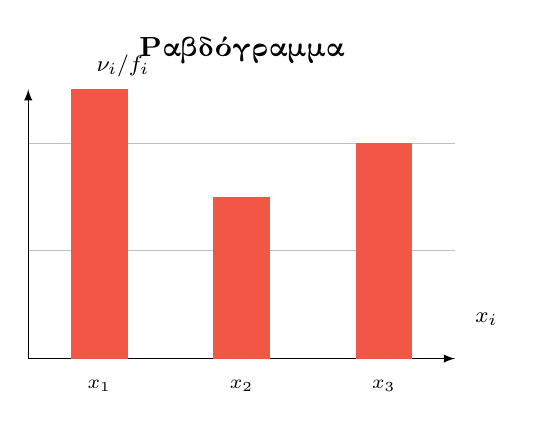
\begin{tikzpicture}
\begin{axis}[axis lines=left,belh ar,
width  = 7cm,
height = 5cm,
major x tick style = transparent,
ybar=2*\pgflinewidth,
bar width=20pt,ylabel={\footnotesize \rotatebox{-90}{$ \nu_i/f_i $}},xlabel={\footnotesize $ x_i $},xlabel style={at={(current axis.right of origin)},xshift=4mm,yshift=5mm, anchor=center},ylabel style={at={(current axis.above origin)},xshift=3mm,yshift=-3mm,,anchor=center},
ymajorgrids = true,
symbolic x coords={$ x_1 $,$ x_2 $,$ x_3 $},
xtick = data,
scaled y ticks = false,
enlarge x limits=0.25,
ymin=0,ymajorticks=false,title={\textbf{Ραβδόγραμμα}},
legend cell align=left,
legend style={at={(1,1.05)},anchor=south east,
column sep=1ex}]
\addplot[style={d,fill=d,mark=none}]
coordinates {($ x_1 $, 5.0) ($ x_2 $,3.0) ($ x_3 $,4.0)};
%\legend{Μαθηματικά,Φυσική,TreeScore $>3$,TreeScore $>4$}
\end{axis}
\end{tikzpicture}\captionof{figure}{Ραβδόγραμμα}
\end{minipage}\hfill
\begin{minipage}{0.48\textwidth}
\centering
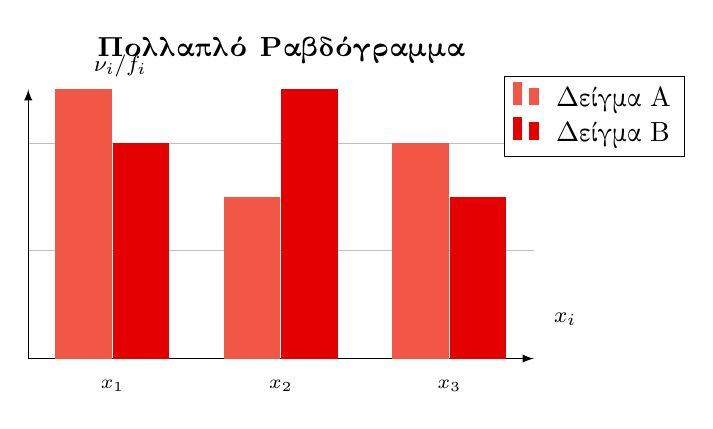
\begin{tikzpicture}
\begin{axis}[axis lines=left,belh ar,
width  = 8cm,
height = 5cm,
major x tick style = transparent,title={\textbf{Πολλαπλό Ραβδόγραμμα}},
ybar=2*\pgflinewidth,
bar width=20pt,ylabel={\footnotesize \rotatebox{-90}{$ \nu_i/f_i $}},xlabel={\footnotesize $ x_i $},xlabel style={at={(current axis.right of origin)},xshift=4mm,yshift=5mm, anchor=center},ylabel style={at={(current axis.above origin)},xshift=3mm,yshift=-1mm,,anchor=center},
ymajorgrids = true,ymajorticks=false,
symbolic x coords={$ x_1 $,$ x_2 $,$ x_3 $},
xtick = data,
scaled y ticks = false,
enlarge x limits=0.25,
ymin=0,
legend cell align=left,
legend style={at={(1.3,1.05)},anchor=north east,
column sep=1ex}]
\addplot[style={d,fill=d,mark=none}]
coordinates {($ x_1 $, 5.0) ($ x_2 $,3.0) ($ x_3 $,4.0)};
\addplot[style={red!90!black,fill=red!90!black,mark=none}]
coordinates {($ x_1 $, 4.0) ($ x_2 $,5.0) ($ x_3 $,3.0)};
\legend{Δείγμα Α,Δείγμα Β}
\end{axis}
\end{tikzpicture}\captionof{figure}{Πολλαπλό ραβδόγραμμα}
\end{minipage}
\end{figure}
\begin{enumerate}[resume]
\item Διάγραμμα : Χρησιμοποιείται για την παράσταση δεδομένων \textbf{ποσοτικής} μεταβλητής.
\item Κυκλικό διάγραμμα : 
\begin{alist}
\item 
Χρησιμοποιείται για την παράσταση δεδομένων τόσο \textbf{ποιοτικής} όσο και \textbf{ποσοτικής} μεταβλητής.
\item Μέτρο τόξου της τιμής $x_i$ σε κυκλικό διάγραμμα : $a_i=\dfrac{\nu_i}{\nu}\cdot 360\degree=f_i\cdot 360\degree$.
\end{alist}
\end{enumerate}
\begin{figure}[!htb]
\begin{minipage}{0.48\textwidth}
\centering
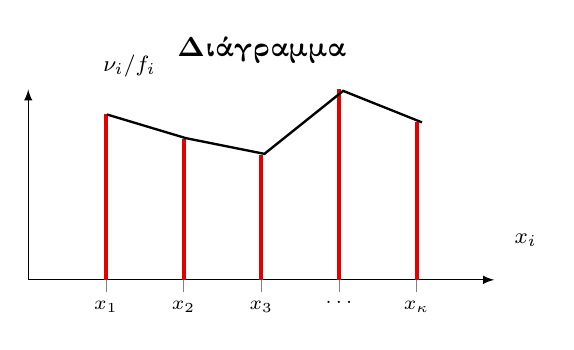
\begin{tikzpicture}
\begin{axis}[axis lines=left,belh ar,ybar,enlarge x limits=0.25,bar width=1pt,ymin=0,ylabel={\footnotesize \rotatebox{-90}{$ \nu_i/f_i $}},xlabel={\footnotesize $ x_i $},xlabel style={at={(current axis.right of origin)},xshift=4mm,yshift=5mm, anchor=center},ylabel style={at={(current axis.above origin)},xshift=3mm,yshift=-3mm,,anchor=center},height=4cm,width=7.5cm,symbolic x coords={$ x_1 $,$ x_2 $,$ x_3 $,$\ldots$,$ x_\kappa $},
xtick = data,ymajorticks=false,title={\textbf{Διάγραμμα}}]
\addplot
[draw=red!90!black,fill=red!90!black] 
coordinates
{($ x_1 $,20) ($ x_2 $,17) ($ x_3 $,15) ($\ldots$,23) ($ x_\kappa $,19)};
\end{axis}
\draw[pl] (1,2.1) -- (2,1.8)-- (3,1.6)-- (4,2.4)-- (5,2);
\end{tikzpicture}\captionof{figure}{Διάγραμμα - Πολύγωνο συχνοτήτων}
\end{minipage}\hfill
\begin{minipage}{0.48\textwidth}
\centering
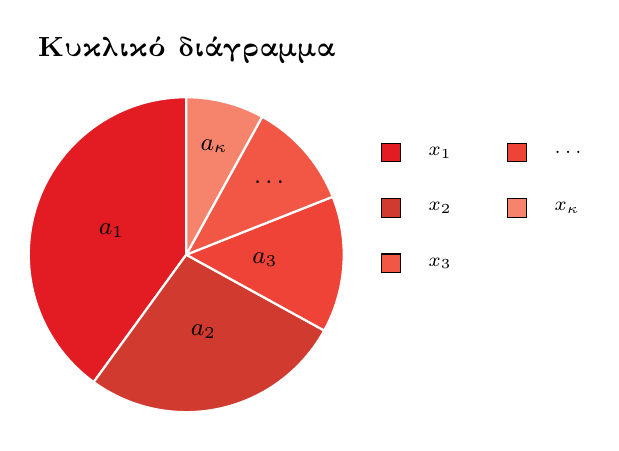
\begin{tikzpicture}
[pie chart,slice type={comet}{a},
slice type={legno}{b},
slice type={coltello}{d},
slice type={sedia}{c},
slice type={caffe}{e},
pie values/.style={font={\small}},
scale=2
]
\node at (0,1.3) {\textbf{Κυκλικό διάγραμμα}};
\pie[values of coltello/.style={pos=.7}]{}{40/comet/a_1,27/legno/a_2,14/sedia/a_3,11/coltello/\ldots,8/caffe/a_\kappa}{100}


\legend[shift={(1.3cm,1cm)}]{{$ x_1 $}/comet, {$ x_2 $}/legno, {$ x_3 $}/coltello}
\legend[shift={(2.1cm,1cm)}]{{$ \ldots $}/sedia, {$ x_\kappa $}/caffe}

\end{tikzpicture}\captionof{figure}{Κυκλικό διάγραμμα συχνοτήτων}
\end{minipage}
\end{figure}
\subsection{Ομαδοποιημένες παρατηρήσεις}
\begin{enumerate}[resume]
\item Εύρος παρατηρήσεων $ R=t_{\max}-t_{\min} $
\item Πλάτος κλάσης $ c=\dfrac{R}{\kappa} $ όπου $ \kappa $ το πλήθος των κλάσεων.
\item Κεντρική τιμή $x_i$ της κλάσης $ [a,\beta) $
\begin{multicols}{2}
\begin{itemize}
\item $ x_i=\dfrac{a+\beta}{2},i=1,\ldots,\kappa $
\item $x_i=x_{i-1}+c,\ i=2,\ldots,\kappa$
\end{itemize}
\end{multicols}
\end{enumerate}
\begin{figure}[!htb]
\begin{minipage}{0.48\textwidth}
\centering
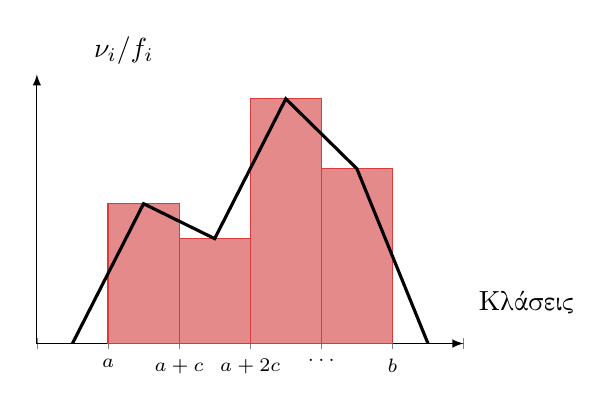
\begin{tikzpicture}
\begin{axis}[axis lines=left,belh ar,width=7cm,
height=5cm,xmin=-2,xmax=10,xlabel style={at={(current axis.right of origin)},xshift=8mm,yshift=5mm, anchor=center},
ylabel style={at={(current axis.above origin)},yshift=-2mm,xshift=3mm,anchor=center},
ymin=0, ymax=7.7,xlabel={Κλάσεις},ylabel={\rotatebox{-90}{$ \nu_i/f_i $}},xticklabels={,,$a$,$a+c$,$a+2c$,$\ldots$,$b$},ymajorticks=false]
\draw[color=red5,fill=red7] (axis cs:0,0) rectangle (axis cs:2,4);
\draw[color=red5,fill=red7] (axis cs:2,0) rectangle (axis cs:4,3);
\draw[color=red5,fill=red7] (axis cs:4,0) rectangle (axis cs:6,7);
\draw[color=red5,fill=red7] (axis cs:6,0) rectangle (axis cs:8,5);
\draw[plm] (axis cs:-1,0)--(axis cs:1,4)--(axis cs:3,3)--(axis cs:5,7)--(axis cs:7,5)--(axis cs:9,0);
\end{axis}
\end{tikzpicture}\captionof{figure}{Ιστόγραμμα - Πολύγωνο συχνοτήτων}
\end{minipage}\hfill
\begin{minipage}{0.48\textwidth}
\centering
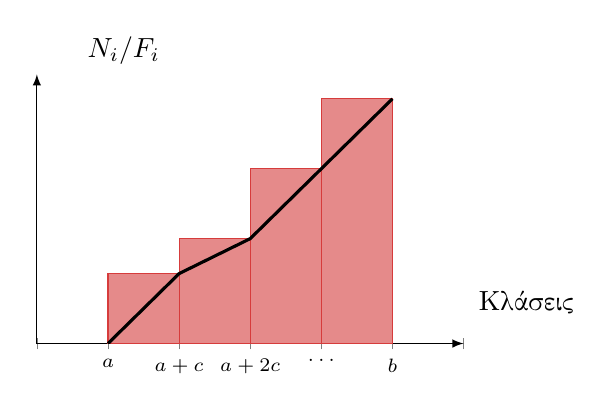
\begin{tikzpicture}
\begin{axis}[axis lines=left,belh ar,width=7cm,
height=5cm,xmin=-2,xmax=10,xlabel style={at={(current axis.right of origin)},xshift=8mm,yshift=5mm, anchor=center},
ylabel style={at={(current axis.above origin)},yshift=-2mm,xshift=3mm,anchor=center},
ymin=0, ymax=7.7,xlabel={Κλάσεις},ylabel={\rotatebox{-90}{$ N_i/F_i $}},xticklabels={,,$a$,$a+c$,$a+2c$,$\ldots$,$b$},ymajorticks=false]
\draw[color=red5,fill=red7] (axis cs:0,0) rectangle (axis cs:2,2);
\draw[color=red5,fill=red7] (axis cs:2,0) rectangle (axis cs:4,3);
\draw[color=red5,fill=red7] (axis cs:4,0) rectangle (axis cs:6,5);
\draw[color=red5,fill=red7] (axis cs:6,0) rectangle (axis cs:8,7);
\draw[plm] (axis cs:0,0)--(axis cs:2,2)--(axis cs:4,3)--(axis cs:6,5)--(axis cs:8,7);
\end{axis}
\end{tikzpicture}\captionof{figure}{Ιστόγραμμα - Πολύγωνο αθροιστικών συχνοτήτων}
\end{minipage}
\end{figure}
\subsection{Μέτρα θέσης}
\begin{enumerate}[resume]
\item Μέση τιμή :
\begin{alist}
\item Με παρατηρήσεις $t_i : \bar{x}=\dfrac{t_1+t_2+\ldots+t_\nu}{\nu}=\dfrac{1}{\nu}\displaystyle\sum\limits_{i=1}^{\nu}{t_i} $
\begin{multicols}{2}
\item Με συχνότητες $\nu_i$ :
$ \bar{x}=\dfrac{1}{\nu}\displaystyle\sum\limits_{i=1}^{\kappa}{x_i\nu_i}$
\item Με συχνότητες $ f_i :  \bar{x}=\displaystyle\sum\limits_{i=1}^{\kappa}{x_if_i} $
\end{multicols}
\end{alist}\label{meshtimh}
\item Σταθμικός μέσος : $\bar{x}=\dfrac{t_iw_1+t_2w_2+\ldots+t_\nu w_\nu}{w_1+w_2+\ldots+w_\nu}=\dfrac{\sum\limits_{i=1}^{\nu}{t_iw_i}}{\sum\limits_{i=1}^{\nu}{w_i}} $
όπου $ w_i\ ,\ i=1,2,\ldots,\nu $ είναι οι συντελεστές βαρύτητας των παρατηρήσεων.\label{stahmikos}
\item Διάμεσος 
\begin{alist}
\begin{multicols}{2}
\item $\delta=t_{\frac{v+1}{2}}$ για $\nu$: περιττό
\item $\delta=\dfrac{t_{\frac{\nu}{2}}+t_{\frac{\nu}{2}+1}}{2}$ για $\nu$: άρτιο
\end{multicols}
\item Διάμεσος σε ομαδοποιημένα δεδομένα
\begin{multicols}{2}
\begin{itemize}
\item 
$\delta=L_i+\dfrac{c}{\nu_i}\left(\dfrac{\nu}{2}-N_{i-1}\right)$.
\item 
$\delta=L_i+\dfrac{c}{f_i\%}\left(50-F_{i-1}\%\right)$.
\end{itemize}
\end{multicols}
όπου $i:$ ο δείκτης της κλάσης στην οποία ξεπερνάμε 1η φορά ή συναντάμε το μισό δείγμα (βλέπε μέθοδο \ref{diamesos1} και \ref{diamesos2})
\end{alist}
\end{enumerate}
\subsection{Μέτρα διασποράς}
\begin{enumerate}[resume]
\item\label{evros} Εύρος
\begin{itemize}
\item Με παρατηρήσεις $t_i$ : $ R=t_{max}-t_{min} $.
\item Από απλό πίνακα συχνοτήτων ή πίνακα ομαδοποιημένων παρατηρήσεων : $ R=x_{max}-x_{min} $.
\end{itemize}
\item Διακύμανση\label{diakymansh}
\begin{alist}
\item Με παρατηρήσεις $t_i$ : $ s^2=\dfrac{1}{\nu}\displaystyle\sum_{i=1}^{\nu}{(t_i-\bar{x})^2} $ για \textbf{ακέραιο} μέσο όρο.
\item Με παρατηρήσεις $t_i$ : $ s^2=\dfrac{1}{\nu}\LEFTRIGHT\{\}{\sum\limits_{i=1}^{\nu}{t_i^2}-\frac{\left( \sum\limits_{i=1}^{\nu}{t_i}\right)^2 }{\nu}} $ για \textbf{μη ακέραιο μέσο} όρο.
\item Με συχνότητα $\nu_i$ : $ s^2=\dfrac{1}{\nu}\displaystyle\sum\limits_{i=1}^{\kappa}{(x_i-\bar{x})^2\nu_i} $ για \textbf{ακέραιο} μέσο όρο.
\item Με συχνότητα $\nu_i$ : $ s^2=\dfrac{1}{\nu}\LEFTRIGHT\{\}{\sum\limits_{i=1}^{\kappa}{x_i^2\nu_i}-\frac{\left( \sum\limits_{i=1}^{\kappa}{x_i\nu_i}\right)^2 }{\nu}} $ για \textbf{μη ακέραιο} μέσο όρο.
\item Με συχνότητα $f_i$ : $ s^2=\displaystyle\sum\limits_{i=1}^{\kappa}{x_i^2f_i-(\bar{x})^2} $
\end{alist}
\item Σχέση μεταξύ διακύμανσης και μέσης τιμής : $s^2=\overline{x^2}-\bar{x}^2$ όπου $\overline{x^2}=\frac{1}{\nu}\displaystyle\sum\limits_{i=1}^{\nu}{t_i^2}$
\item Τυπική απόκλιση $ s=\sqrt{s^2} $
\item Συντελεστής μεταβλητότητας $ CV=\dfrac{s}{|\overline{x}|} $
\begin{itemize}
\item Αν $CV\leq 10\%$ τότε το δείγμα είναι ομοιογενές.
\item Αν $CV_A<CV_B$ τότε το δείγμα $A$ έχει μεγαλύτερη ομοιογένεια από το $B$.
\end{itemize}
\item Κανονική κατανομή
\begin{center}
\begin{tikzpicture}
\begin{axis}[axis y line=none,aks_on,belh ar,
no markers,xmax=8, samples=200,
axis lines*=left, xlabel=$x_i$, ylabel=$\nu_i$,
every axis y label/.style={at=(current axis.above origin),anchor=south},ymin=0,
every axis x label/.style={at=(current axis.right of origin),anchor=west},
height=4.5cm, width=12cm,xticklabels={$ \bar{x}-3s $,$ \bar{x}-2s $,$ \bar{x}-s $,$ \bar{x} $,$ \bar{x}+s $,$ \bar{x}+2s $,$ \bar{x}+3s $},  xtick={1,2,3,4,5,6,7},enlargelimits=false, clip=false, axis on top]
\addplot [thick,fill=red!10,domain=0:1] {gauss(4,1)+0.015} \closedcycle;\addplot [fill=red!30, domain=1:2] {gauss(4,1)+0.015} \closedcycle;
\addplot [fill=red!10, domain=2:3] {gauss(4,1)+0.015} \closedcycle;
\addplot [fill=red!30, domain=3:4] {gauss(4,1)+0.015} \closedcycle;
\addplot [fill=red!30, domain=4:5] {gauss(4,1)+0.015} \closedcycle;
\addplot [fill=red!10, domain=5:6] {gauss(4,1)+0.015} \closedcycle;
\addplot [fill=red!30, domain=6:7] {gauss(4,1)+0.015} \closedcycle;
\addplot [fill=red!10, domain=7:8] {gauss(4,1)+0.015} \closedcycle;
\addplot [plm,draw=red!80!black,domain=0:8] {gauss(4,1)+0.015};
\node at (axis cs:3.5,0.15){\footnotesize$34\%$};
\node at (axis cs:4.5,0.15){\footnotesize$34\%$};
\node at (axis cs:5.5,0.05){\footnotesize$13{,}5\%$};
\node at (axis cs:6.5,0.08){\footnotesize$2{,}35\%$};
\node at (axis cs:7.5,0.08){\footnotesize$0{,}15\%$};
\node at (axis cs:2.5,0.05){\footnotesize$13{,}5\%$};
\node at (axis cs:1.5,0.08){\footnotesize$2{,}35\%$};
\node at (axis cs:0.5,0.08){\footnotesize$0{,}15\%$};
\draw[{Bar[]latex[]}-{latex[]Bar[]}] (axis cs:3,-.09)--(axis cs:5,-.09)node[pos=0.5,below] {$68\%$};
\draw[{Bar[]latex[]}-{latex[]Bar[]}] (axis cs:2,-.17)--(axis cs:6,-.17)node[pos=0.5,below] {$95\%$};
\draw[{Bar[]latex[]}-{latex[]Bar[]}] (axis cs:1,-.25)--(axis cs:7,-.25)node[pos=0.5,below] {$99{,}7\%$};
\end{axis}
\end{tikzpicture}\captionof{figure}{Κανονική κατανομή}
\end{center}
\item Μεταβολές των παρατηρήσεων\\
Δίνονται οι παρατηρήσεις $x_1,x_2,\ldots,x_\nu$ μιας μεταβλητής $X$, με μέση τιμή $\bar{x}$ και τυπική απόκλιση $s_x$. Οι μεταβολές στις τιμές αυτές  επηρεάζουν τη μέση τιμή και την τυπική απόκλιση σύμφωνα με τον ακόλουθο πίνακα.
\begin{center}
\begin{mytblr}{}
Αλλαγή & Τελικές τιμές & Νέα μέση τιμή & Νέα τυπική απόκλιση\\
Αύξηση - Μείωση & $y_i=x_i\pm c$ & $\bar{y}=\bar{x}\pm c$ & $s_y=s_x$\\
Πολλαπλασιασμός & $y_i=x_i\cdot c$ & $\bar{y}=\bar{x}\cdot c$ & $s_y=s_x\cdot |c|$\\
Διαίρεση & $y_i=\dfrac{x_i}{c}$ & $\bar{y}=\dfrac{\bar{x}}{c}$ & $s_y=\dfrac{s_x}{|c|}$\\
Αύξηση κατά $a\%$ & $y_i=x_i\left(1+a\%\right)$ & $\bar{y}=\bar{x}\left(1+a\%\right)$ & $s_y=s_x\left(1+a\%\right)$\\
Μείωση κατά $a\%$ & $y_i=x_i\left(1-a\%\right)$ & $\bar{y}=\bar{x}\left(1-a\%\right)$ & $s_y=s_x\left(1-a\%\right)$\\
Μέρος & $y_i=x_i\cdot a\%$ & $\bar{y}=\bar{x}\cdot a\%$ & $s_y=s_x\cdot a\%$\\
Συνδυασμός & $y_i=\lambda\cdot x_i\pm c$ & $\bar{y}=\lambda\cdot\bar{x}\pm c$ & $s_y=|\lambda|s_x$\\
\end{mytblr}\captionof{table}{Υπολογισμός νέας μέσης τιμής και τυπικής απόκλισης από μεταβολές παρατηρήσεων}\label{pinakas3}
\end{center}
\end{enumerate}
\newpage
\renewcommand{\myleftmark}{{\large Βασικά είδη ασκήσεων}}
\newpage
\begin{center}
\part{Βασικά είδη ασκήσεων}
\end{center}
\section{Διαφορικός λογισμός}
\begin{askhsh}{Εύρεση πεδίου ορισμού}
Επιλέγουμε, σύμφωνα με τον πίνακα \ref{pinakas}, τους απαραίτητους περιορισμούς. Το πεδίο ορισμού προκύπτει από τη συναλήθευση όλων των περιορισμών.
\end{askhsh}
\noindent
\Paradeigma{Πεδίο ορισμού}
\bmath{Να βρεθεί το πεδίο ορισμού των παρακάτω συναρτήσεων
\begin{alist}
\begin{multicols}{2}
\item $f(x)=\dfrac{x^2}{x-2}$
\item $f(x)=\sqrt{9-3x}$
\item $f(x)=\dfrac{2x+5}{\sqrt{x^2-3x+2}}$
\item $f(x)=\dfrac{1}{x-3}+\sqrt{x-2}$
\end{multicols}
\end{alist}}
\lysh\vspace{-5mm}
\begin{alist}
\item Για να ορίζεται η συνάρτηση $f$ πρέπει
\[ x-2\neq 0\Rightarrow x\neq 2 \]
άρα το πεδίο ορισμού της είναι $D_f=\mathbb{R}-\{2\}$.
\item Η συνάρτηση $f$ ορίζεται όταν 
\[ 9-3x\geq 0\Rightarrow -3x\geq -9\Rightarrow \frac{-3x}{-3}\leq \frac{-9}{-3}\Rightarrow x\leq 3 \]
άρα το πεδίο ορισμού της είναι $D_f=(-\infty,3]$.
\item Για να ορίζεται η $f$ πρέπει
\begin{gather*}
x^2-3x+2>0\\
\varDelta=\beta^2-4a\gamma=(-3)^2+4\cdot 1\cdot 2=9-8=1>0\\
x_{1,2}=\frac{-\beta\pm\sqrt{\varDelta}}{2a}=\frac{-(-3)\pm\sqrt{1}}{2\cdot1}=\frac{3\pm1}{2}
\end{gather*}
\wrapr{-15mm}{5}{7cm}{5mm}{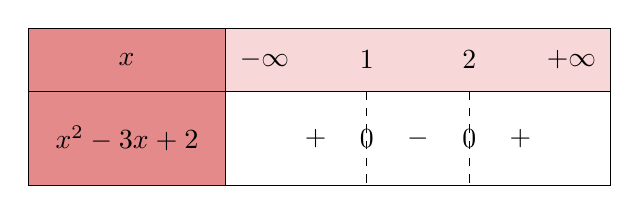
\begin{tikzpicture}
\tikzset{t style/.style = {style = dashed}}
\tikzset{z style/.style = {fill=white,inner sep=.2mm}}
\tkzTabInit[color,lgt=2.5,espcl=1.3,colorC = red7,
colorL = red9,
colorV = red7]%
{$x$ / .8,$x^2-3x+2$ /1.2}%
{$-\infty$,$1$,$2$,$+\infty$}%
\tkzTabLine{ , +, z
, -, z
, +, }
\end{tikzpicture}}{
\begin{multicols}{2}
\begin{itemize}
\item $x_1=\dfrac{3+1}{2}=\dfrac{4}{2}=2$
\item $x_2=\dfrac{3-1}{2}=\dfrac{2}{2}=1$
\end{itemize}
\end{multicols}
Επομένως, σύμφωνα με το διπλανό πίνακα προσήμων, το πεδίο ορισμού της $f$ είναι $D_f=(-\infty,1)\cup(2,\infty)$.}
\item Ο τύπος της συνάρτησης περιέχει και κλάσμα και ρίζα. Επομένως για να ορίζεται η $f$ πρέπει να ισχύουν συγχρόνως
\begin{itemize}
\item $x-3\neq 0\Rightarrow x\neq 3$ και
\item $x-2\geq 0\Rightarrow x\geq 2$
\end{itemize}
Για τους περιορισμούς αυτούς βρίσκουμε τις κοινές τιμές του $x$ που τους επαληθεύουν οπότε θα έχει πεδίο ορισμού $D_f=[2,3)\cup(3,+\infty)$.
\end{alist}
\begin{askhsh}{Σημεία τομής με τους άξονες}
Για να βρούμε τα σημεία τομής της γραφικής παράστασης $C_f$ μιας συνάρτησης $f$ με τον
\begin{itemize}
\item άξονα $x'x$, λύνουμε την εξίσωση $f(x)=0$.
\item άξονα $y'y$, υπολογίζουμε, αν ορίζεται, το $f(0)$.
\end{itemize}
\end{askhsh}
\noindent
\Paradeigma{Σημεία τομής της $C_f$ με τους άξονες}
\bmath{Να βρεθούν τα σημεία τομής της γραφικής παράστασης της συνάρτησης $f(x)=x^3+2x^2-x-2$ με τους άξονες $x'x$ και $y'y$.}\\
\lysh
\wrapr{-5mm}{7}{5.8cm}{-5mm}{
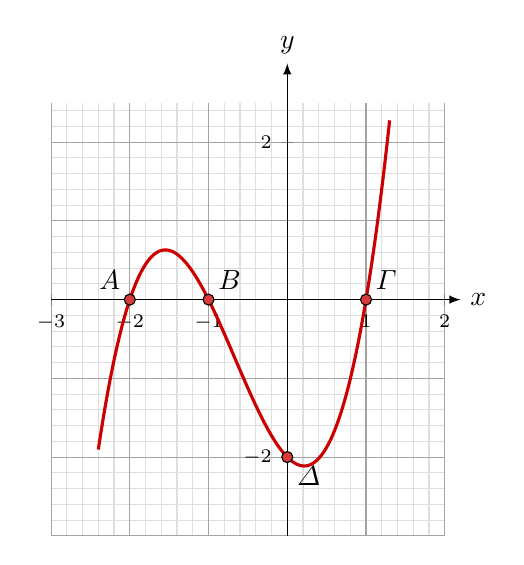
\begin{tikzpicture}
\draw [step=0.2,gray9] (0,0) grid (5,5.5);
\draw [step=1.0,gray7] (0,0) grid (5,5.5);
\begin{axis}[aks_on,belh ar,xmin=-3,xmax=2.2,ymin=-3,ymax=3,xlabel=$x$,ylabel=$y$,x=1cm,y=1cm]
\addplot[pl,grafikh parastash,domain=-2.4:1.3] {x^3+2*x^2-x-2};
\draw[fill=red5] (axis cs:-2,0) circle (2pt) node[anchor=south east]{$A$};
\draw[fill=red5] (axis cs:-1,0) circle (2pt) node[anchor=south west]{$B$};
\draw[fill=red5] (axis cs:1,0) circle (2pt) node[anchor=south west]{$\varGamma$};
\draw[fill=red5] (axis cs:0,-2) circle (2pt) node[anchor=north west]{$\varDelta$};
\end{axis}
\end{tikzpicture}}{Η συνάρτηση $f$ ορίζεται στο $\mathbb{R}$.
\begin{itemize}
\item Λύνουμε την εξίσωση:
\begin{gather*}
f(x)=0\Rightarrow x^3+2x^2-x-2=0\Rightarrow\\
x^2(x+2)-(x+2)=0\Rightarrow\\
(x+2)(x^2-1)=0\Rightarrow
\end{gather*}
\begin{itemize}
\item $x+2=0\Rightarrow x=-2$ ή 
\item $x^2-1=0\Rightarrow x^2=1\Rightarrow |x|=1\Rightarrow x=\pm 1$
\end{itemize}
Επομένως η $C_f$ τέμνει τον $x'x$ στα σημεία $A(-2,0),B(-1,0)$ και $\varGamma(-1,0)$.
\item Για $x=0$ είναι $f(0)=0^3+2\cdot0^2-0-2=-2$ άρα η $C_f$ τέμνει τον άξονα $y'y$ στο σημείο $\varDelta(0,-2)$.
\end{itemize}}
\begin{askhsh}{Όριο της μορφής $\frac{0}{0}$ σε σημείο $ x_0 $}
\begin{itemize}
\item Αν η συνάρτηση είναι ρητή τότε παραγοντοποιούμε τα πολυώνυμα ώσπου να εμφανιστεί η παράσταση $ x-x_0 $ και να απλοποιηθεί.
\item Αν η συνάρτηση περιέχει ρίζα, πολλαπλασιάζουμε πάνω και κάτω με τη συζυγή παράσταση του όρου που έχει τη ρίζα. Στη συνέχεια κάνουμε πράξεις μέχρι να διαιρεθεί η παράσταση $x-x_0$. Τέλος υπολογίζουμε το όριο.
\end{itemize}
\end{askhsh}\mbox{}\\
\Paradeigma{Όριο $\frac{0}{0}$ ρητής συνάρτησης}
\bmath{Να υπολογίσετε το όριο
\[ \lim_{x\to 1}{\frac{x^3-3x+2}{x^2-1}} \]}
\lysh
Για το όριο της συνάρτησης $f(x)=\frac{x^3-3x+2}{x^2-1},\ x\neq \pm1$ στο σημείο $x=1$ έχουμε:
\begin{align*}
\lim\limits_{x\to 1}{f(x)}&=\lim_{x\to 1}{\frac{x^3-3x+2}{x^2-1}}\stackrel{\frac{0}{0}}{=}\lim_{x\to 1}{\frac{(x-1)\left(x^2+x-2\right)}{(x-1)(x+1)}}=\\
&=\lim_{x\to 1}{\frac{x^2+x-2}{x+1}}=\frac{0}{2}=0
\end{align*}
\Paradeigma{Όριο $\frac{0}{0}$ άρρητης συνάρτησης}
\bmath{Να υπολογίσετε το όριο
\[ \lim_{x\to 3}{\frac{\sqrt{x+1}-2}{x^2-9}} \]}
\lysh
Η συνάρτηση $f(x)=\frac{\sqrt{x+1}-2}{x^2-9}$ ορίζεται στο $D_f=[-1,3)\cup(3,+\infty)$. Έχουμε
\begin{align*}
\lim\limits_{x\to 3}{f(x)}&=\lim_{x\to 3}{\frac{\sqrt{x+1}-2}{x^2-9}}\stackrel{\frac{0}{0}}{=}\lim_{x\to 3}{\frac{\left(\sqrt{x+1}-2\right)\left(\sqrt{x+1}+2\right)}{\left(x^2-9\right)\left(\sqrt{x+1}+2\right)}}=\\
&=\lim_{x\to 3}{\frac{\sqrt{x+1}^2-2^2}{(x+3)(x-3)\left(\sqrt{x+1}+2\right)}}=\lim_{x\to 3}{\frac{x-3}{(x+3)(x-3)\left(\sqrt{x+1}+2\right)}}=\\&=\lim_{x\to 3}{\frac{1}{(x+3)\left(\sqrt{x+1}+2\right)}}=\frac{1}{24}
\end{align*}
\begin{askhsh}{Συνέχεια συνάρτησης σε σημείο}
\begin{alist}
\item Υπολογίζουμε το όριο της $ f $ στο σημείο $ x_0 $: $\lim\limits_{x\to x_0}{f(x)}$
\item Υπολογίζουμε την τιμή $f(x_0)$.
\end{alist}
Αν είναι ίσα τότε η συνάρτηση είναι συνεχής στο $x_0$.
\end{askhsh}\mbox{}\\
\Paradeigma{Έλεγχος συνέχειας}
\bmath{Να εξετάσετε αν η συνάρτηση
\[ f(x)=\begin{cdcases}
x^2-3x+4 & ,x\neq 1\\2 & ,x=1
\end{cdcases} \]
είναι συνεχής στο σημείο $x_0=1$.}\\
\lysh
Από το 2ο κλάδο της $f$ φαίνεται αμέσως ότι $f(1)=2$. Επίσης
\begin{align*}
\lim_{x\to 1}{f(x)}&=\lim_{x\to 1}{(x^2-3x+4)}=1^2-3\cdot 1+4=2
\end{align*}
Άρα $\lim\limits_{x\to 1}{f(x)}=f(1)=2$ οπότε η $f$ είναι συνεχής στο σημείο $x=1$.\\
\Paradeigma{Συνέχεια συνάρτησης - Εύρεση παραμέτρου}
\bmath{Δίνεται συνεχής συνάρτηση $f:\mathbb{R}\to\mathbb{R}$ με τύπο
\[ f(x)=\begin{cdcases}
\frac{x^2+ax-a-1}{x+1} & , x\neq-1\\
a-2 & ,x=-1
\end{cdcases} \]
Να υπολογίσετε την τιμή της παραμέτρου $a\in\mathbb{R}$.}\\
\lysh
Αφού η $f$ είναι συνεχής, τότε θα είναι συνεχής και στο $x=-1$ που σημαίνει
\[ \lim_{x\to-1}{f(x)}=f(-1) \]
\begin{itemize}
\item $f(-1)=a-2$.
\item $\begin{aligned}[t]
\lim\limits_{x\to-1}{f(x)}&=\lim\limits_{x\to-1}{\frac{x^2+ax-a-1}{x+1}}=\\&=\lim\limits_{x\to-1}{\frac{(x-1)(x+1)-a(x+1)}{x+1}}=\lim\limits_{x\to-1}{\frac{(x+1)(x-1-a)}{x+1}}=\\&=\lim\limits_{x\to-1}{(x-1-a)}=-2-a
\end{aligned}$
\end{itemize}
Επομένως προκύπτει η εξίσωση
\begin{gather*}
a-2=-2-a\Rightarrow 2a=0\Rightarrow a=0
\end{gather*}
\begin{askhsh}{Παράγωγος απλών - σύνθετων συναρτήσεων}
Για να υπολογίσουμε τις παραγώγους απλών ή και σύνθετων συναρτήσεων ακολουθούμε τον πίνακα \ref{pinakas1} καθώς και τους κανόνες παραγώγισης πίνακα \ref{pinakas2} για τις πράξεις.
\end{askhsh}\mbox{}\\
\Paradeigma{Υπολογισμός απλών παραγώγων}
\bmath{Να υπολογίσετε τις παραγώγους των συναρτήσεων
\begin{multicols}{2}
\begin{alist}
\item $f(x)=3x^4-5x^3+\sqrt{x}-\hm{x}$
\item $f(x)=\ef{x}-\frac{4}{x}+\sqrt{3}$
\item $f(x)=x^2\cdot\hm{x}$
\item $f(x)=\dfrac{x^3-x}{x+3}$
\end{alist}
\end{multicols}}
\noindent
\lysh
\vspace{-5mm}
\begin{alist}
\item Για να ορίζεται η $f$ πρέπει $x\geq 0$ άρα $D_f=[0,+\infty)$. Για κάθε $x\in(0,+\infty)$ :
\begin{align*} f'(x)&=\left(3x^4-5x^3+\sqrt{x}-\hm{x}\right)'=\\&=\left(3x^4\right)'-\left( 5x^3\right) '+\left( \sqrt{x}\right) -(\hm{x})'=\\&=12x^3-15x^2+\frac{1}{2\sqrt{x}}-\syn{x}
\end{align*}
\item Η $f$ ορίζεται όταν $x\neq0$ άρα $D_f=\mathbb{R}^*$. Για κάθε $x\neq 0$ : 
\[ f'(x)=\left(\ef{x}-\frac{4}{x}+\sqrt{3}\right)'=\left(\ef{x}\right)' -\left(\frac{4}{x}\right)' +\left( \sqrt{3}\right)'=\frac{1}{\syn^2{x}}+\frac{4}{x^2} \]
\item Η $f$ ορίζεται στο $D_f=\mathbb{R}$. Για κάθε $x\in\mathbb{R}$ 
\[f'(x)=(x^2\cdot\hm{x})'=(x^2)'\cdot\hm{x}+x^2\cdot(\hm{x})'=2x\cdot\hm{x}+x^2\cdot\syn{x}\]
\item Η $f$ ορίζεται όταν $x-3\neq 0\Rightarrow x\neq 3$ άρα $D_f=\mathbb{R}-\{3\}$. Για κάθε $x\in D_f$ : 
\begin{align*}
f'(x)&=\left(\frac{x^3-x}{x+3}\right)'=\frac{(x^3-x)'(x+3)-(x^3-x)(x+3)'}{(x+3)^2}=\\
&=\frac{(3x^2-1)(x+3)-(x^3-x)}{(x+3)^2}=\\
&=\frac{3x^3-9x^2-x-3-x^3+x}{(x+3)^2}=\frac{2x^3-9x^2-3}{(x+3)^2}
\end{align*}
\end{alist}
\Paradeigma{Υπολογισμός σύνθετων παραγώγων}
\bmath{Να υπολογίσετε τις παραγώγους των συναρτήσεων
\begin{multicols}{2}
\begin{alist}
\item $f(x)=\left(x^2-4x\right)^5$
\item $f(x)=\hm{\left(x^3\right)}\ ,\ x\in\left(0,\frac{\pi}{2}\right)$
\item $f(x)=\sqrt{x^2-2x}$
\item $f(x)=\dfrac{3}{\syn{x}}\ ,\ x\in\left(0,\frac{\pi}{2}\right)$
\end{alist}
\end{multicols}}
\noindent
\lysh
\vspace{-5mm}
\begin{alist}
\item Η $f$ ορίζεται στο $D_f=\mathbb{R}$. Για κάθε $x\in\mathbb{R}$ 
\[f'(x)=\left[(x^2-4x)^5\right]'=5(x^2-4x)^5\cdot(x^2-4x)'=5(x^2-4x)^5(2x-4)\]
\item Για κάθε $x\in D_f$ έχουμε: 
\[f'(x)=\left[\hm{\left(x^3\right)}\right]'=\syn{\left(x^3\right)}\cdot\left(x^3\right)'=3x^2\syn{\left(x^3\right)}\]
\item Για να ορίζεται η $f$ πρέπει 
\[x^2-2x\geq 0\Rightarrow x\in(-\infty,0]\cup[2,+\infty)\]
Για κάθε $x\in (-\infty,0)\cup (2,+\infty)$ :
\begin{align*}
f'(x)&=(\sqrt{x^2-2x})'=\frac{(x^2-2x)'}{2\sqrt{x^2-2x}}=\\&=\frac{2x-2}{2\sqrt{x^2-2x}}=\frac{x-1}{\sqrt{x^2-2x}}
\end{align*}
\item Για κάθε $x\in\left(0,\frac{\pi}{2}\right)$ :
\[f'(x)=\left(\frac{3}{\syn{x}}\right)'=-\frac{3(\syn{x})'}{\syn^2{x}}=-\frac{3\hm{x}}{\syn^2{x}}\]
\end{alist}
\noindent
\begin{askhsh}{Εφαπτομένη της $C_f$ όταν γνωρίζουμε το σημείο επαφής $ M(x_0,f(x_0))$}
\begin{alist}
\item Υπολογίζουμε την $f'(x)$.
\item Υπολογίζουμε την τιμή $f(x_0)$ και την $f'(x_0)$ που είναι ο συντελεστής διεύθυνσης της εφαπτομένης.
\item Τοποθετούμε στην εξίσωση $y=\lambda x+\beta$ όπου $\lambda=f'(x_0)$.
\item Αντικαθιστούμε στην εξίσωση τις συντεταγμένες του σημείου $A(x_0,f(x_0))$ στη θέση των μεταβλητών $x,y$ και λύνοντας την, υπολογίζουμε το $\beta$.
\item Γράφουμε την εξίσωση της ευθείας.
\end{alist}
\end{askhsh}
\noindent
\Paradeigma{Εφαπτομένη σε γνωστό σημείο}
\bmath{Να βρείτε την εξίσωση της εφαπτομένης της γραφικής παράστασης της $f(x)=\dfrac{x^2}{x-2}$ στο σημείο $A(3,f(3))$.}\\
\lysh
Η συνάρτηση $f$ ορίζεται όταν $x-2\neq 0\Rightarrow x\neq 2$ άρα $D_f=\mathbb{R}-\{2\}$. Για κάθε $x\in D_f$ :
\begin{align*}
f'(x)&=\left(\frac{x^2}{x-2}\right)'=\frac{(x^2)'(x-2)-x^2(x-2)'}{(x-2)^2}=\\&=\frac{2x(x-2)-x^2}{(x-2)^2}=\frac{x^2-4x}{(x-2)^2}
\end{align*}
Θέτοντας λοιπόν $x=3$ έχουμε
\begin{itemize}[itemsep=0mm]
\item $f(3)=\dfrac{3^2}{3-2}=9$
\item $f'(3)=\dfrac{3^2-4\cdot 3}{(3-2)^2}=-3$
\end{itemize}
Η εξίσωση της ευθείας δίνεται από τον τύπο
\[y=\lambda x+\beta\Rightarrow y=-3x+\beta\]
Αφού το σημείο $A(3,9)$ ανήκει στην ευθεία, τότε οι συντεταγμένες του επαληθεύουν την εξίσωσή της. Άρα για $x=3$ και $y=9$ έχουμε
\[9=-3\cdot 3+\beta\Rightarrow 9=-9+\beta\Rightarrow \beta=18\]
Επομένως η εξίσωση της ευθείας είναι $y=-3x+18$.
\begin{askhsh}{Εφαπτομένη της $C_f$ όταν γνωρίζουμε την κλίση της ευθείας}
\begin{alist}
\item Θεωρούμε σημείο επαφής $A(x_0,f(x_0))$.
\item Υπολογίζουμε την $f'(x)$.\\
\wrapr{-10mm}{9}{7.7cm}{-5mm}{\begin{parat}{8.3cm}
\begin{itemize}[label=\faCaretSquareRight,leftmargin=3mm,itemsep=0mm]
\item Δύο ευθείες παράλληλες έχουν ίσους συντελεστές διεύθυνσης: $\varepsilon_1\parallel\varepsilon_2\Rightarrow\lambda_1=\lambda_2$.
\item Για δύο κάθετες ευθείες ισχύει $\lambda_1\cdot\lambda_2=-1$.
\item Οι ευθείες παράλληλες με τον άξονα $x'x'$ έχουν $\lambda=0$.
\item Αν η ευθεία σχηματίζει γωνία $\omega$ με τον άξονα $x'x'$ τότε $\lambda=\ef{\omega}$.
\end{itemize}
\end{parat}}{
\item Υπολογίζουμε, αν δεν μας δίνεται, το συντελεστή διεύθυνσης $\lambda$ της εφαπτομένης. \textcolor{red!80!black}{\faLightbulb[regular]}
\item Λύνουμε την εξίσωση $f'(x_0)=\lambda$ και βρίσκουμε το $x_0$ και στη συνέχεια το $f(x_0)$.
\item Τοποθετούμε στην εξίσωση $y=\lambda x+\beta$ όπου $\lambda=f'(x_0)$.
\item Αντικαθιστούμε στην εξίσωση τις συντεταγμένες του $A(x_0,f(x_0))$ στη θέση των μεταβλητών $x,y$ και λύνοντας την υπολογίζουμε το $\beta$.
\item Γράφουμε την εξίσωση της ευθείας.}
\end{alist}
\end{askhsh}
\noindent
\Paradeigma{Εφαπτομένη με γνωστή κλίση}
\bmath{Δίνεται η συνάρτηση $f(x)=x^2-x-2$. Να βρεθεί η εφαπτομένη της $C_f$ η οποία
\begin{multicols}{2}
\begin{alist}
\item έχει συντελεστή διεύθυνσης $\lambda=3$.
\item είναι παράλληλη με την ευθεία $\zeta : y=-x+2$.
\item είναι κάθετη στην ευθεία $\eta : y=\frac{x}{5}+1$.
\item σχηματίζει γωνία $\omega=45\degree$ με τον $x'x$.
\end{alist}
\end{multicols}}
\noindent
\lysh
Η συνάρτηση $f$ ορίζεται στο $\mathbb{R}$. Έστω $A(x_0,f(x_0))$ το σημείο επαφής. Για κάθε $x\in\mathbb{R}$ επίσης έχουμε
\[ f'(x)=\left(x^2-x-2\right)'=2x-1 \]
\begin{alist}
\item Η ζητούμενη εφαπτομένη έχει συντελεστή διεύθυνσης $\lambda=3$ επομένως :
\[ \lambda=3\Rightarrow f'(x_0)=3\Rightarrow 2x_0-1=3\Rightarrow x_0=2 \]
Για $x_0=2$ λοιπόν είναι $f(2)=2^2-2-2=0$. Η εξίσωση της ευθείας δίνεται από τον τύπο
\[y=\lambda x+\beta\Rightarrow y=2x+\beta\]
Αφού το σημείο $A(2,0)$ ανήκει στην ευθεία τότε για $x=2$ και $y=0$ έχουμε
\[0=2\cdot 2+\beta\Rightarrow 0=4+\beta\Rightarrow \beta=-4\]
Επομένως η εξίσωση της ευθείας είναι $y=2x-4$.
\item Η δοσμένη ευθεία έχει συντελεστή διεύθυνσης $\lambda_{\zeta}=-1$ ενώ η ζητούμενη εφαπτομένη $\varepsilon $ έχει $\lambda_{\varepsilon}=f'(x_0)$. Αφού $\varepsilon\parallel \zeta$ τότε
\[ \lambda_{\varepsilon}=\lambda_{\zeta}\Rightarrow f'(x_0)=-1\Rightarrow 2x_0-1=-1\Rightarrow x_0=0 \]
Θέτοντας $x_0=0$ θα είναι $f(0)=0^2-0-2=-2$. Η εξίσωση της ευθείας δίνεται από τον τύπο
\[y=\lambda x+\beta\Rightarrow y=-x+\beta\]
Αφού το σημείο $A(0,-2)$ ανήκει στην ευθεία τότε για $x=0$ και $y=-2$ έχουμε
\[-2=-1\cdot 0+\beta\Rightarrow \beta=-2\]
Άρα η εξίσωση της ευθείας είναι $y=-x-2$.
\item Η ευθεία $\eta$ έχει συντελεστή διεύθυνσης $\lambda_{\eta}=\frac{1}{5}$ ενώ η εφαπτομένη $\varepsilon $ έχει $\lambda_{\varepsilon}=f'(x_0)$. Αφού $\varepsilon\perp \eta$ τότε
\[ \lambda_{\varepsilon}\cdot\lambda_{\eta}=-1\Rightarrow f'(x_0)\cdot\frac{1}{5}=-1\Rightarrow f'(x_0)=-5\Rightarrow 2x_0-1=-5\Rightarrow x_0=-2 \]
Θέτοντας $x_0=-2$ έχουμε $f(-2)=(-2)^2-(-2)-2=4$. Η ζητούμενη ευθεία έχει εξίσωση
\[y=\lambda x+\beta\Rightarrow y=-5x+\beta\]
Αφού το σημείο $A(-2,4)$ ανήκει στην ευθεία τότε για $x=-2$ και $y=4$ έχουμε
\[4=-5\cdot(-2)+\beta\Rightarrow 4=10+\beta\Rightarrow \beta=-6\]
Άρα η εξίσωση της ευθείας είναι $y=-5x-6$.
\item Η εφαπτομένη είναι παράλληλη με τον άξονα $x'x$ άρα έχει συντελεστή διεύθυνσης $\lambda=0$. Συνεπώς :
\[ \lambda=0\Rightarrow f'(x_0)=0\Rightarrow 2x_0-1=0\Rightarrow x_0=\frac{1}{2} \]
Για $x_0=\frac{1}{2}$ λοιπόν είναι $f\left(\frac{1}{2}\right)=\left(\frac{1}{2}\right)^2-\frac{1}{2}-2=-\frac{9}{4}$. Η εξίσωση της ευθείας δίνεται από τον τύπο
\[y=\lambda x+\beta\Rightarrow y=\beta\]
Αφού το σημείο $A\left(\frac{1}{2},-\frac{9}{4}\right)$ ανήκει στην ευθεία τότε για $x=\frac{1}{2}$ και $y=-\frac{9}{4}$ έχουμε $\beta=-\frac{9}{4}$
άρα η εξίσωση της ευθείας είναι $y=-\frac{9}{4}$.
\end{alist}
\begin{askhsh}{Μονοτονία - Ακρότατα}
\begin{alist}
\item Βρίσκουμε το πεδίο ορισμού της $f$ και ελέγχουμε αν είναι συνεχής.
\item Υπολογίζουμε την $f'(x)$.
\item Λύνουμε την εξίσωση $f'(x)=0$.
\item Λύνουμε τις ανισώσεις $f'(x)>0$ και $f'(x)<0$.
\item Σχηματίζουμε και συμπληρώνουμε πίνακα προσήμων της $f'$ και μονοτονίας της $f$.
\item Απαντάμε για το είδος της μονοτονίας σε κάθε διάστημα καθώς και για το είδος και τη θέση των ακρότατων εκεί που αλλάζει η μονοτονία.
\end{alist}
\end{askhsh}
\noindent
\Paradeigma{Μονοτονία - Ακρότατα}
\bmath{Να μελετσετε τη συνάρτηση $f(x)=x^2-4x+3$ ως προς τη μονοτονία και τα ακρότατα.}\\
\lysh
Η συνάρτηση $f$ ορίζεται στο $\mathbb{R}$ στο οποίο είναι συνεχής ως πολυωνυμική. Για κάθε $x\in\mathbb{R}$ είναι :
\[ f'(x)=\left(x^2-4x+2\right)'=2x-4 \]
Έστω λοιπόν
\begin{itemize}[itemsep=0mm]
\item $f'(x)=0\Rightarrow 2x-4=0\Rightarrow 2x=4\Rightarrow x=2$
\item $f'(x)>0\Rightarrow 2x-4>0\Rightarrow 2x>4\Rightarrow x>2$
\item $f'(x)<0\Rightarrow 2x-4<0\Rightarrow 2x<4\Rightarrow x<2$
\end{itemize}
Στον παρακάτω πίνακα βλέπουμε τα πρόσημα της $f'$ καθώς και τη μονοτονία και τα ακρότατα της $f$.
\begin{center}
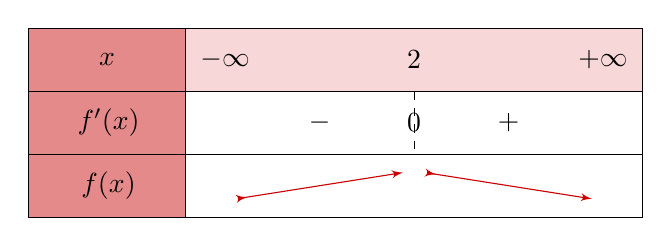
\begin{tikzpicture}
\tikzset{arrow style/.style=
{red!80!black,>->,>=latex'}
}
\tikzset{t style/.style = {style = dashed}}
\tikzset{z style/.style = {inner sep=.2mm}}
\tkzTabInit[color,lgt=2,espcl=2.4,colorC = red7,
colorL = red9,
colorV = red7]%
{$x$ / .8,$f'(x)$ /.8,$f(x)$/0.8}%
{$-\infty$,$2$,$+\infty$}%
\tkzTabLine{,-,z,+,}
\tkzTabVar{-/,+/,-/}
\end{tikzpicture}
\end{center}
Η συνάρτηση $f$ είναι γνησίως αύξουσα στο διάστημα $[2,+\infty)$ και γνησίως φθίνουσα στο $(-\infty,2]$. Επίσης παρουσιάζει τοπικό ελάχιστο στη θέση $x=2$ το οποίο ισούται με $f(2)=-1$.
\begin{askhsh}{Ρυθμός μεταβολής}
Όταν ζητείται ο ρυθμός μεταβολής μιας συνάρτησης $f$ τότε υπολογίζουμε την παράγωγο $f'$ της $f$. Αν ζητάμε το ρυθμό μεταβολής της $f$ σε ένα σημείο $x_0$ τότε υπολογίζουμε το $f'(x_0)$. Σε αρκετά προβλήματα πρέπει να κατασκευάσουμε εμείς τον τύπο της $f$.
\end{askhsh}\mbox{}\\
\Paradeigma{Ρυθμός μεταβολής - Γεωμετρία}
\bmath{Δίνεται ορθογώνιο παραλληλόγραμμο $AB\varGamma\varDelta$ με σταθερή περίμετρο $20$ \si{\centi\meter} και μήκος $AB=x$ \si{\centi\meter}.
\begin{alist}
\item Να εκφράσετε το πλάτος του ορθογωνίου ως συνάρτηση του $x$.
\item Βρείτε το ρυθμό μεταβολής του εμβαδού του ορθογωνίου, ως προς $x$, όταν $x=3$ \si{\centi\meter}.
\end{alist}
}
\lysh
\wrapr{-11mm}{8}{4.5cm}{4mm}{
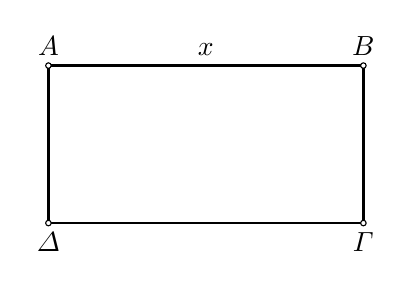
\begin{tikzpicture}
\tkzDefPoints{0/2/A,4/2/B,4/0/C,0/0/D}
\draw[pl] (D) rectangle (B);
\tkzDrawPoint[fill=white](A);
\tkzDrawPoint[fill=white](B);
\tkzDrawPoint[fill=white](C);
\tkzDrawPoint[fill=white](D);
\tkzLabelPoint[above](A){$A$}
\tkzLabelPoint[above](B){$B$}
\tkzLabelPoint[below](C){$\varGamma$}
\tkzLabelPoint[below](D){$\varDelta$}
\tkzText[yshift=2mm](2,2){$x$}
\end{tikzpicture}
}{
\begin{alist}
\item Γνωρίζουμε ότι η περίμετρος του ορθογωνίου είναι $20\si{\centi\meter} $. Θα είναι λοιπόν
\begin{gather*}
AB+B\varGamma+\varGamma\varDelta+\varDelta A=20\Rightarrow\\
x+B\varGamma+x+B\varGamma=20\Rightarrow\\
2B\varGamma=20-2x\Rightarrow B\varGamma=10-x
\end{gather*}
\end{alist}
}
\begin{alist}[start=2]
\item Το εμβαδόν του ορθογωνίου δίνεται από τον τύπο
\begin{align*}
E&=AB\cdot B\varGamma=x(10-x)=-x^2+10x
\end{align*}
Επιπλέον πρέπει να ισχύει $x>0$ καθώς και $10-x>0\Rightarrow x<10$. Οπότε
\[ E(x)=-x^2+10x\ ,\ x\in(0,10) \]
Για κάθε $x\in(0,10)$ έχουμε
\[ E'(x)=\left(-x^2+10x\right)'=-2x+10 \]
άρα ο ρυθμός μεταβολής του εμβαδού του ορθογωνίου, ως προς $x$ όταν $x=3\si{\centi\meter}$ ισούται με $Ε'(3)=-2\cdot 3+10=4$.
\end{alist}
\begin{askhsh}{Σύγκριση αριθμών με τη βοήθεια μονοτονίας}
Αν μας ζητείται να συγκρίνουμε δύο τιμές $f(a)$ και $f(\beta)$, με $a<\beta$, της συνάρτησης $f$ τότε μελετάμε την $f$ ως προς τη μονοτονία της. 
\begin{itemize}
\item Αν $f\nearrow$ τότε $a<\beta\Rightarrow f(a)<f(\beta)$
\item Αν $f\searrow$ τότε $a<\beta\Rightarrow f(a)>f(\beta)$.
\end{itemize}
\end{askhsh}
\noindent
\Paradeigma{Σύγκριση τιμών συνάρτησης}
\bmath{Δίνεται η συνάρτηση $f(x)=\dfrac{2x}{x^2+1}$.
\begin{alist}
\item Να μελετήσετε την $f$ ως προς τη μονοτονία.
\item Να συγκρίνετε τους αριθμούς $f\left(\frac{9}{17}\right)$ και $f\left(\frac{11}{20}\right)$.
\end{alist}}
\noindent\lysh
\begin{alist}
\item Για να ορίζεται η $f$ πρέπει να ισχύει $x^2+1\neq 0\Rightarrow x\in\mathbb{R}$. Για κάθε $x\in\mathbb{R}$ έχουμε
\begin{align*}
f'(x)&=\left(\frac{2x}{x^2+1}\right)'=\frac{(2x)'(x^2+1)-2x(x^2+1)'}{(x^2+1)^2}=\\
&=\frac{2(x^2+1)-2x\cdot 2x}{(x^2+1)^2}=\frac{2x^2+2-4x^2}{(x^2+1)^2}=\frac{2-2x^2}{(x^2+1)^2}
\end{align*}
Λύνουμε την εξίσωση 
\[ f'(x)=0\Rightarrow\frac{2-2x^2}{(x^2+1)^2}=0\Rightarrow 2x^2=2\Rightarrow x^2=1\Rightarrow x=\pm 1\]
Στη συνέχεια λύνουμε τις ανισώσεις
\[ f'(x)>0\Rightarrow\frac{2-2x^2}{(x^2+1)^2}>0\Rightarrow 2-2x^2>0\Rightarrow x^2<1\Rightarrow -1<x<1 \]
και
\[ f'(x)<0\Rightarrow\frac{2-2x^2}{(x^2+1)^2}<0\Rightarrow 2-2x^2<0\Rightarrow x^2>1\Rightarrow x<-1\ \textrm{ή}\ x>1 \]
Στον παρακάτω πίνακα βλέπουμε τα πρόσημα της $f'$ και τη μονοτονία της $f$.
\begin{center}
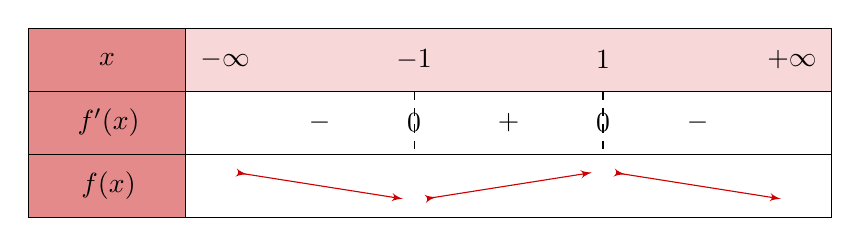
\begin{tikzpicture}
\tikzset{arrow style/.style=
{red!80!black,>->,>=latex'}
}
\tikzset{t style/.style = {style = dashed}}
\tikzset{z style/.style = {fill=white,inner sep=.2mm}}
\tkzTabInit[color,lgt=2,espcl=2.4,colorC = red7,
colorL = red9,
colorV = red7]%
{$x$ / .8,$f'(x)$ /.8,$f(x)$/0.8}%
{$-\infty$,$-1$,$1$,$+\infty$}%
\tkzTabLine{,-,z,+,z,-,}
\tkzTabVar{+/,-/,+/,-/}
\end{tikzpicture}
\end{center}
Η συνάρτηση $f$ είναι γνησίως αύξουσα στο διάστημα $[-1,1]$ και γνησίως φθίνουσα στα $(-\infty,-1]$ και $[1,+\infty)$.
\item Παρατηρούμε ότι οι αριθμοί $\frac{9}{17}$ και $\frac{11}{20}$ ανήκουν στο διάστημα $[-1,1]$ στο οποίο η $f$ είναι γνησίως αύξουσα. Επομένως
\[ \frac{9}{17}<\frac{11}{20}\Rightarrow f\left(\frac{9}{17}\right)<f\left(\frac{11}{20}\right) \]
\end{alist}
\begin{askhsh}{Απόδειξη ανισότητας με τη βοήθεια ακρότατων}
Αν μας ζητείται να αποδείξουμε μια ανισότητα της μορφής $f(x)\leq a$ ή $f(x)\geq a$ τότε μελετάμε τη συνάρτηση ως προς τα ακρότατα της.
\begin{itemize}
\item Αν η συνάρτηση παρουσιάζει μέγιστο το $a$ στη θέση $x_0$ τότε από τον ορισμό του μέγιστου γράφουμε $f(x)\leq f(x_0)\Rightarrow f(x)\leq a$.
\item Αν η συνάρτηση παρουσιάζει ελάχιστο το $a$ στη θέση $x_0$ τότε από τον ορισμό του μέγιστου γράφουμε $f(x)\geq f(x_0)\Rightarrow f(x)\geq a$.
\end{itemize}
\end{askhsh}
\noindent
\Paradeigma{Απόδειξη ανισότητας}
\bmath{Δίνεται η συνάρτηση $f(x)=\sqrt{4x-x^4}$
\begin{alist}
\item Να μελετήσετε την $f$ ως προς τα ακρότατα.
\item Να αποδείξετε ότι $4x\leq x^4+3$ για κάθε $x\in D_f$.
\end{alist}}
\noindent
\lysh
\begin{alist}
\item Η συνάρτηση $f$ ορίζεται όταν
\[ 4x-x^4\geq 0\Rightarrow x\in[0,\sqrt[3]{4}] \]
Για κάθε $x\in(0,\sqrt[3]{4})$ έχουμε
\begin{align*}
f'(x)&=\left(\sqrt{4x-x^4}\right)'=\frac{\left(4x-x^4\right)'}{2\sqrt{4x-x^4}}=\\&=\frac{4-4x^3}{2\sqrt{4x-x^4}}=\frac{4(1-x^3)}{2\sqrt{4x-x^4}}=\frac{2(1-x^3)}{\sqrt{4x-x^4}}
\end{align*}
Υπολογίζουμε στη συνέχεια ρίζες και πρόσημα της $f'$:
\begin{itemize}
\item $f'(x)=0\Rightarrow\frac{2(1-x^3)}{\sqrt{4x-x^4}}=0\Rightarrow 2(1-x^3)=0\Rightarrow x=1$
\item $f'(x)>0\Rightarrow\frac{2(1-x^3)}{\sqrt{4x-x^4}}>0\Rightarrow 2(1-x^3)>0\Rightarrow x<1\Rightarrow x\in(0,1)$
\item $f'(x)<0\Rightarrow\frac{2(1-x^3)}{\sqrt{4x-x^4}}<0\Rightarrow 2(1-x^3)<0\Rightarrow x>1\Rightarrow x\in(1,\sqrt[3]{4})$
\end{itemize}\mbox{}\\
\wrapr{-5mm}{8}{7cm}{-7mm}{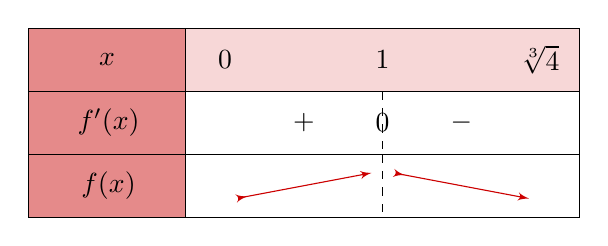
\begin{tikzpicture}
\tikzset{arrow style/.style=
{red!80!black,>->,>=latex'}
}
\tikzset{t style/.style = {style = dashed}}
\tkzTabInit[color,lgt=2,espcl=2,colorC = red7,
colorL = red9,
colorV = red7]%
{$x$ / .8,$f'(x)$ /0.8,$ f(x) $/0.8}%
{$0$,$ 1 $,$\sqrt[3]{4}$}%
\tkzTabLine{,+,z,-,}
\tkzTabVar{-/,+/,-/}
\draw[dashed](4.5,-1.6)--(4.5,-2.4);
\end{tikzpicture}}{Στο διπλανό πίνακα μονοτονίας και ακροτάτων βλέπουμε ότι η $f$ παρουσιάζει ολικό μέγιστο στη θέση $x=2$ το οποίο είναι $f(1)=\sqrt{3}$. Επίσης παρουσιάζει ολικό ελάχιστο στις θέσεις $x=0$ και $x=\sqrt[3]{4}$ το $f(0)=f(\sqrt[3]{4})=0$
\item Σύμφωνα με τη μελέτη ακροτάτων που κάναμε προηγουμένως και σύμφωνα με τον ορισμό του ολικού μέγιστου θα ισχύει}
\begin{align*}
f(x)\leq f(1)&\Rightarrow \sqrt{4x-x^2}\leq \sqrt{3} \Rightarrow\\&\Rightarrow 4x-x^4\leq 3\Rightarrow 4x\leq x^4+3\ ,\ \text{για κάθε }x\in[0,\sqrt[3]{4}] 
\end{align*}
\end{alist}
\newpage
\section{Στατιστική}
\begin{askhsh}{Συμπλήρωση πίνακα συχνοτήτων}
\begin{itemize}
\item Χρησιμοποιούμε τις ιδιότητες των συχνοτήτων $\nu_i,f_i,f_i\%,N_i,F_i,F_i\%$ από το τυπολόγιο. Κάθε τύπος είναι εξίσωση από την οποία βρίσκουμε διαδοχικά τις συχνότητες που λείπουν από τον πίνακα.
\item Κάθε συχνότητα που βρίσκουμε την συμπληρώνουμε στον πίνακα. Οι πράξεις γίνονται κάτω από τον πίνακα.
\end{itemize}
\end{askhsh}
\noindent
\Paradeigma{Συμπλήρωση πίνακα}\label{Parad:Sympl_Pinaka}
\bmath{Ρωτήσαμε σε ένα δείγμα από ελληνικές οικογένειες πόσα παιδιά έχουν. Να συμπληρώσετε τον παρακάτω πίνακα συχνοτήτων
\begin{center}
\begin{mytblr}{columns = {8mm,c},column{1} = {18mm,c},row{1}={m}}
{Πλήθος\\παιδιών $x_i$} & $\nu_i$ & $f_i$ & $f_i\%$ & $N_i$ & $F_i$ & $F_i\%$ \\ 
$0$ & $8$ &  &  &  &  &  \\
$1$ &  & $0{,}2$ &  & $18$ &  &  \\
$2$ &  &  &  &  &  &  \\
$3$ &  &  & $22$ &  &  &  \\
Σύνολο &  &  &  & \SetCell{bg=gray7} & \SetCell{bg=gray7} &  \SetCell{bg=gray7}
\end{mytblr}\captionof{table}{Πλήθος παιδιών στις ελληνικές οικογένειες}
\end{center}
}
\noindent\lysh
Σύμφωνα με την υπόθεση της άσκησης γνωρίζουμε τα εξής στοιχεία του πίνακα : $\nu_1=8,f_2=0{,}2,f_4\%=22$ και $N_2=18$. Έχουμε λοιπόν :
\begin{center}
\begin{mytblr}{columns = {8mm,c},column{1} = {18mm,c},row{1}={m}}
{Πλήθος\\παιδιών \bmath{$x_i$}} & \bmath{$\nu_i$} & $f_i$ & $f_i\%$ & $N_i$ & $F_i$ & $F_i\%$ \\ 
$0$ & $8$ & \bmath{$0{,}16$} & \bmath{$16$} & \bmath{$8$} & \bmath{$0{,}16$} & \bmath{$16$} \\
$1$ & \bmath{$10$} & $0{,}2$ & \bmath{$20$} & $18$ & \bmath{$0{,}36$} & \bmath{$36$} \\
$2$ & \bmath{$21$} & \bmath{$0{,}42$} & \bmath{$42$} & \bmath{$39$} & \bmath{$0{,}78$} & \bmath{$78$} \\
$3$ & \bmath{$11$} & \bmath{$0{,}22$} & $22$ & \bmath{$50$} & \bmath{$1$} & \bmath{$100$} \\
Σύνολο & \bmath{$50$} & \bmath{$1$} & \bmath{$100$} & \SetCell{bg=gray7} & \SetCell{bg=gray7} &  \SetCell{bg=gray7}
\end{mytblr}
\end{center}
\begin{multicols}{2}
\begin{itemize}
%\begin{minipage}{0.6\linewidth}
\item $\nu_1=N_1=8$
\item $\nu_2=N_2-N_1=18-8=10$
\item $f_2=\dfrac{\nu_2}{\nu}\Rightarrow 0{,}2=\dfrac{10}{\nu}\Rightarrow 0{,}2\nu=10\Rightarrow \nu=50$
\item $f_4\%=f_4\cdot 100\Rightarrow 22=f_4\cdot 100\Rightarrow f_4=0{,}22$
\item $f_4=\dfrac{\nu_4}{\nu}\Rightarrow 0{,}22=\dfrac{\nu_4}{50}\Rightarrow \nu_4=11$
\item $\nu_1+\nu_2+\nu_3+\nu_4=\nu\\\Rightarrow 8+10+\nu_3+11=50\Rightarrow\nu_3=21$
\item $f_1=\dfrac{\nu_1}{\nu}=\dfrac{8}{50}=0{,}16$
\item $f_1=F_1=0{,}16$
\item $f_3=\dfrac{\nu_3}{\nu}=\dfrac{21}{50}=0{,}42$
\item $N_3=N_2+\nu_3=18+21=39$
%\end{minipage}
%\begin{minipage}{0.4\linewidth}
\item $N_4=\nu=50$
\item $f_1\%=f_1\cdot 100=0{,}16\cdot 100=16$
\item $f_2\%=f_2\cdot 100=0{,}2\cdot 100=20$
\item $f_3\%=f_3\cdot 100=0{,}42\cdot 100=42$
\item $F_2=f_1+f_2=0{,}16+0{,}2=0{,}36$
\item $F_3=F_2+f_3=0{,}36+0{,}42=0{,}78$
\item $F_4=1$
\item $F_1\%=f_1\%=16$
\item $F_2\%=F_2\cdot 100=0{,}36\cdot 100=36$
\item $F_3\%=F_3\cdot 100=0{,}78\cdot 100=78$
\item $F_4\%=100$
%\end{minipage}
\end{itemize}
\end{multicols}
\begin{askhsh}{Συμπλήρωση πίνακα ομαδοποιημένων παρατηρήσεων}
Ο πίνακας συχνοτήτων ομαδοποιημένων παρατηρήσεων συμπληρώνεται ακριβώς όπως και ο συνήθης πίνακας υπολογίζοντας τις συχνότητες που περιέχει. Αν επιπλέον λείπουν από τον πίνακα και τα άκρα των κλάσεων καθώς και οι κεντρικές τιμές τότε
\begin{alist}
\item Θέτουμε με $ a $ το κάτω άκρο της 1ης κλάσης (ή οποιασδήποτε άλλης αν γίνεται) και χρησιμοποιώντας το πλάτος $ c $ των κλάσεων, σχηματίζουμε τις κλάσεις με τον ακόλουθο τρόπο
\[ [a,a+c),[a+c,a+2c),[a+2c,a+3c),\ldots \]
έως ότου συμπληρωθούν όλες οι κλάσεις.
\item Από τα δεδομένα του πίνακα σχηματίζουμε $ 2 $ εξισώσεις με μεταβλητές $ a,c $ και λύνοντας το σύστημα υπολογίζουμε τις τιμές των μεταβλητών αυτών.
\item Στη συνέχεια σχηματίζουμε με τις τιμές αυτές τις ομάδες του πίνακα και συμπληρώνουμε και τις κεντρικές τιμές $ x_i $.
\end{alist}
\end{askhsh}
\noindent
\Paradeigma{Συμπλήρωση πίνακα με ομάδες}\label{Parad:Omadopoihsh}
\bmath{Μετρήσαμε το χρόνο αναμονής (σε λεπτά) $200$ πελατών μιας τράπεζας. Οι παρατηρήσεις έχουν ομαδοποιηθεί σε $4$ κλάσεις ίσου πλάτους. Να συμπληρώσετε τον παρακάτω πίνακα συχνοτήτων
\begin{center}
\begin{mytblr}{columns = {8mm,c},column{1} = {18mm,c},row{1}={m}}
{Χρόνος\\ανανομής} & $x_i$ & $\nu_i$ & $f_i$ & $f_i\%$ & $N_i$ & $F_i$ & $F_i\%$ \\ 
$[\ldots,\ldots)$ & &  & $0{,}1$ &  &  &  &  \\
$[\ldots,\ldots)$ & $15$ & $ 52 $ &  &  & $ $ &  &  \\
$[20,\ldots)$ & &  &  &  & $140$ &  &  \\
$[\ldots,\ldots)$ & &  &  &  &  &  &  \\
Σύνολο & \SetCell{bg=gray7}  & $200$ &  &  & \SetCell{bg=gray7} &  \SetCell{bg=gray7} & \SetCell{bg=gray7}
\end{mytblr}\captionof{table}{Χρόνος αναμονής πελατών σε μια τράπεζα}
\end{center}}
\lysh
Έστω $a$ το κάτω άκρο της 1ης κλάσης και $c$ το πλάτος των κλάσεων. Σχηματίζοντας τις κλάσεις καθώς και τις κεντρικές τιμές τους παίρνουμε αντίστοιχα
\begin{gather*}
[a,a+c),[a+c,a+2c),[a+2c,a+3c),[a+3c,a+4c) \textrm{ καθώς και}\\
x_1=\frac{2a+c}{2},x_2=\frac{2a+3c}{2},x_3=\frac{2a+5c}{2},x_4=\frac{2a+7c}{2}
\end{gather*}
Σύμφωνα με τα δεδομένα της άσκησης προκύπτουν λοιπόν οι εξισώσεις
\[a+2c=20 \textrm{ και } x_2=15\Rightarrow \frac{2a+3c}{2}=15\Rightarrow 2a+3c=30\]
Παίρνουμε έτσι το ακόλουθο γραμμικό σύστημα 
\[ \systeme{a+2c=20,2a+3c=30}\Rightarrow a=0 \textrm{ και }c=10 \]
Υπολογίζουμε έτσι τις ομάδες, τις κεντρικές τιμές τους και συμπληρώνουμε τον πίνακα όπως και στο προηγούμενο παράδειγμα.
\begin{center}
\begin{mytblr}{columns = {8mm,c},column{1} = {18mm,c},row{1}={m}}
\textbf{Χρόνος\\αναμονής} & $x_i$ & $\nu_i$ & $f_i$ & $f_i\%$ & $N_i$ & $F_i$ & $F_i\%$ \\ 
$[0,10)$ & $5$ & $20$ & $0{,}1$ & $10$ & $20$ & $0{,}1$ & $10$ \\
$[10,20)$ & $15$ & $ 52 $ & $0{,}26$ & $26$ & $ 72 $ & $0{,}36$ & $36$ \\
$[20,30)$ & $25$ & $68$ & $0{,}34$ & $34$ & $140$ & $0{,}7$ & $70$ \\
$[30,40)$ & $35$ & $60$ & $0{,}3$ & $30$ & $200$ & $1$ & $100$ \\
Σύνολο & \SetCell{bg=gray7}  & $200$ & $1$ & $100$ & \SetCell{bg=gray7} &  \SetCell{bg=gray7} & \SetCell{bg=gray7}
\end{mytblr}\captionof{table}{Χρόνος αναμονής πελατών στην τράπεζα}
\end{center}
\begin{askhsh}{Συμπεράσματα από πίνακα συχνοτήτων}
Αν ύστερα από τη συμπλήρωση ενός πίνακα καλούμαστε να απαντήσουμε σε ερωτήσεις που αφορούν το δείγμα τότε διακρίνουμε τις εξής περιπτώσεις:
\begin{itemize}
\item Αν οι ερωτήσεις ζητούν \textbf{πλήθος} παρατηρήσεων τότε χρησιμοποιούμε τις συχνότητες $ \nu_i,N_i $.
\item Αν οι ερωτήσεις ζητούν \textbf{ποσοστό} παρατηρήσεων τότε χρησιμοποιούμε τις σχετικές συχνότητες $ f_i\%,F_i\% $.
\end{itemize}
Εάν η ερώτηση αφορά μια τιμή $ x_i $ τότε χρειαζόμαστε την αντίστοιχη συχνότητά $ \nu_i $ ή $ f_i\% $. Αν αφορά πολλές τιμές τότε προσθέτουμε τις αντίστοιχες συχνότητες ή χρησιμοποιούμε κάποια αθροιστική.
\end{askhsh}
\noindent
\Paradeigma{Συμπεράσματα που αφορούν πίνακα συχνοτήτων}
\bmath{Για τον πίνακα του παραδείγματος \ref{Parad:Sympl_Pinaka} που αφορά την έρευνα για το πλήθος παιδιών στις ελληνικές οικογένειες, να απαντήσετε στις ακόλουθες ερωτήσεις.
\begin{alist}
\item Πόσες οικογένειες έχουν τουλάχιστον $2$ παιδιά?
\item Τι ποσοστό οικογενειών έχει το πολύ $1$ παιδί?
\item Πόσες οικογένειες έχουν $1$ ή $2$ παιδιά?
\end{alist}}
\lysh
\begin{alist}
\vspace{-5mm}
\item Η ερώτηση αφορά την 3η και την 4η τιμή της μεταβλητής άρα σύμφωνα με τα στοιχεία του πίνακα το πλήθος των οικογενειών με τουλάχιστον $2$ παιδιά είναι
\[ \nu_3+\nu_4=21+11=32\textrm{ οικογένειες.} \]
\item Εδώ χρειαζόμαστε τις σχετικές συχνότητες από την 1η και 2η τιμή του πίνακα. Επομένως το ζητούμενο ποσοστό θα είναι $F_2\%=36\%$.
\item Ομοίως με πριν το πλήθος των οικογενειών θα είναι 
\[ \nu_2+\nu_3=10+18=28\textrm{ οικογένειες.} \]
\end{alist}
\begin{askhsh}{Συμπεράσματα από πίνακα συχνοτήτων ομαδοποιημένων παρατηρήσεων}
Για να απαντήσουμε σε ερωτήσεις που αφορούν ένα ομαδοποιημένο δείγμα διακρίνουμε τις περιπτώσεις που είδαμε πριν για πλήθος και ποσοστό. Στη συνέχεια ακολουθούμε τις παρακάτω οδηγίες.
\begin{itemize}
\item Κάθε ερώτηση αφορά πλήθος ή ποσοστό παρατηρήσεων μέχρι κάποια τιμή $ x $ (το πολύ $x$), από κάποια τιμή $ x $ (τουλάχιστον $x$) ή μεταξύ δύο τιμών $ x,y $. Αν οι τιμές αυτές
\begin{itemize}
\item είναι \textbf{άκρα} κλάσεων, τότε τις κλάσεις που χρειαζόμαστε τις παίρνουμε ολόκληρες.
\item είναι \textbf{κεντρικές τιμές} κλάσεων, τότε τις κλάσεις που τις περιέχουν τις παίρνουμε μισές.
\item είναι \textbf{τυχαία ενδιάμεσα} σημεία τότε παίρνουμε το \textbf{μέρος} της ομάδας που περιέχει τις τιμές που θέλουμε.
\end{itemize}
\end{itemize}
Αν η τιμή $ x $ περιέχεται στην ομάδα $ [a,\beta) $ αναλυτικά η διαδικασία έχει ως εξής.
\begin{itemize}
\item Η ομάδα χωρίζεται στα διαστήματα $ [a,x) $ και $ [x,\beta) $.
\item Ο παρακάτω πίνακας μας δίνει το μέρος της ομάδας που χρειαζόμαστε
\begin{center}
\begin{mytblr}{}
\textbf{Ζητούμενο} & \textbf{Διάστημα} & \textbf{Μέρος της ομάδας} \\
μέχρι $ x $ & $ [a,x) $ & $ \dfrac{x-a}{c} $ \\[1mm]
από $ x $ & $ [x,\beta) $ & $ \dfrac{\beta-x}{c} $
\end{mytblr}
\end{center}
\item Υποθέτουμε ότι οι παρατηρήσεις είναι ομοιόμορφα κατανεμημένες στην κλάση και πολλαπλασιάζουμε το κλάσμα της 3ης στήλης με τη συχνότητα $ \nu_i $ ή $ f_i $ της κλάσης.
\end{itemize}
\end{askhsh}
\Paradeigma{Συμπεράσματα από ομαδοποιημένο δείγμα}
\bmath{Απαντήστε στις παρακάτω ερωτήσεις που αφορούν τον πίνακα του παραδείγματος \ref{Parad:Omadopoihsh} για το χρόνο αναμονής των πελατών σε μια τράπεζα.
\begin{alist}
\item Πόσοι πελάτες περίμεναν στην ουρά το πολύ $20$ λεπτά?
\item Τι ποσοστό των πελατών περίμενε στην ουρά τουλάχιστον $15$ λεπτά?
\item Τι ποσοστό πελατών περίμενε από $8$ έως $24$ λεπτά?
\end{alist}}
\lysh\vspace{-7mm}
\begin{alist}
\item Παρατηρούμε ότι ο αριθμός $20$ αποτελεί το πάνω άκρο της 2ης κλάσης. Αφού ζητείται το πλήθος των πελατών που περίμεναν \textbf{μέχρι} $20$ λεπτά τότε η ερώτηση αυτή αφορά τις $2$ πρώτες κλάσεις. Έτσι το ζητούμενο πλήθος θα είναι $Ν_2=72$ πελάτες.
\item Τα $15$ λεπτά είναι η κεντρική τιμή της 2ης κλάσης η οποία τη χωρίζει στα διαστήματα $[10,15)$ και $[15,20)$. Οι πελάτες περίμεναν \textbf{τουλάχιστον} $15$ λεπτά οπότε χρειαζόμαστε το 2ο μισό : $[15,20)$. Υποθέτουμε ότι οι παρατηρήσεις είναι ομοιόμορφα κατανεμημένες στις κλάσεις και έτσι το ζητούμενο ποσοστό θα είναι
\[ \frac{f_2\%}{2}+f_3\%+f_4\%=\frac{26}{2}+34+30=77\% \]
\item Οι αριθμοί $8$ και $24$ λεπτά είναι τυχαία ενδιάμεσα σημεία της 1ης και 3ης κλάσης αντίστοιχα. Έτσι υποθέτουμε και εδώ ότι οι παρατηρήσεις είναι ομοιόμορφα κατανεμημένες στις κλάσεις. Θα δούμε λοιπόν κάθε αριθμός σε ποια διαστήματα χωρίζει την κλάση και τι μέρος της είναι το διάστημα που χρειαζόμαστε.
\begin{itemize}
\item Το $8$ χωρίζει την 1η κλάση στα $[0,8)$ και $[8,10)$. Σύμφωνα με την υπόθεση χρειαζόμαστε το διάστημα $[8,10)$ το οποίο είναι το
\[ \frac{10-8}{10}=\frac{2}{10}=\frac{1}{5}\textrm{ της κλάσης} \]
\item Το $24$ χωρίζει την 3η κλάση στα $[20,24)$ και $[24,30)$. Εμείς θα εργαστούμε στο διάστημα $[20,24)$ το οποίο είναι τα
\[ \frac{24-20}{10}=\frac{4}{10}=\frac{2}{5}\textrm{ της κλάσης} \]
\end{itemize}
Έτσι το ζητούμενο ποσοστό των πελατών θα είναι
\[ \frac{1}{5}\cdot f_1\%+f_2\%+\frac{2}{5}\cdot f_3\%=\frac{10}{5}+26+\frac{68}{5}=41{,}6 \]
\end{alist}
\begin{askhsh}{Γραφική παράσταση δεδομένων}
\wrapr{-7mm}{5}{8cm}{-12mm}{\begin{mytblr}{columns = {45mm,c},column{1} = {35mm,c},rows={m},row{odd} = {ht=4mm},
 row{even} = {ht=4mm},}
Σχήμα & {Είδος μεταβλητής}\\
Ραβδόγραμμα & Ποιοτική\\ 
Διάγραμμα & Ποσοτική\\
{Κυκλικό διάγραμμα} & {Ποιοτική και ποσοτική}\\ 
Ιστόγραμμα & {Ποσοτική (ομαδοποιημένα δεδομένα)}
\end{mytblr}}{
Για τη γραφική παράσταση δεδομένων, επιλέγουμε το κατάλληλο σχήμα ανάλογα με τον τύπο της μεταβλητής που εξετάζουμε (ποιοτική ή ποσοτική). Τα κυριότερα σχήματα είναι το ραβδόγραμμα, το διάγραμμα, το κυκλικό διάγραμμα και το ιστόγραμμα. Ακολουθούμε τον οδηγό στο διπλανό πίνακα.}
\end{askhsh}
\Paradeigma{Ραβδόγραμμα συχνοτήτων}
\wrapr{-5mm}{13}{3.5cm}{-5mm}{
\begin{mytblr}{columns = {8mm,c},column{1} = {18mm,c},row{1}={m},row{odd} = {ht=4mm},
 row{even} = {ht=4mm},}
{Μέσο \bmath{$x_i$}} & \bmath{$\nu_i$}\\
Λεωφορείο & $ 58 $\\ 
Αυτοκίνητο & $90$\\
Μηχανή & $ 44 $\\ 
Ταξί & $ 18 $\\
\textbf{Σύνολο} & \bmath{$200$} 
\end{mytblr}}{
\bmath{Ρωτήσαμε $200$ υπαλλήλους μιας εταιρίας τι μεταφορικό μέσο χρησιμοποιούν για να πάνε στη δουλειά. Τα αποτελέσματα φαίνονται στο διπλανό πίνακα συχνοτήτων. Να κατασκευάσετε ραβδόγραμμα σχετικών συχνοτήτων για τα δεδομένα αυτά.}\\
\lysh
Θα υπολογίσουμε αρχικά τη σχετική συχνότητα κάθε τιμής. Έχουμε λοιπόν:
\begin{multicols}{2}
\begin{itemize}
\item $f_1=\dfrac{\nu_1}{\nu}=\dfrac{58}{200}=0{,}29$
\item $f_2=\dfrac{\nu_2}{\nu}=\dfrac{90}{200}=0{,}45$
\item $f_3=\dfrac{\nu_3}{\nu}=\dfrac{44}{200}=0{,}22$
\item $f_4=\dfrac{\nu_4}{\nu}=\dfrac{18}{200}=0{,}09$
\end{itemize}
\end{multicols}}
\wrapl{5mm}{7}{7cm}{-11mm}{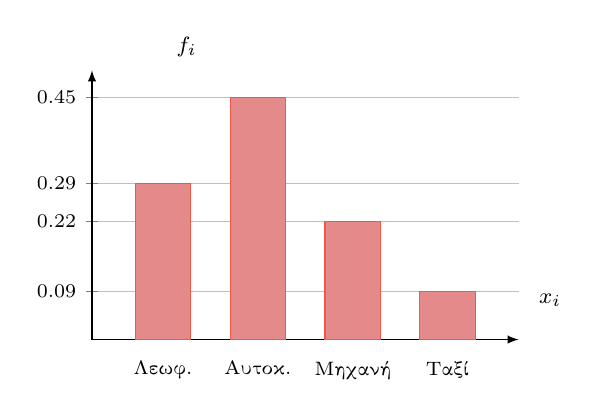
\begin{tikzpicture}
\begin{axis}[axis lines=left,belh ar,
width  = 7cm,
height = 5cm,
major x tick style = transparent,
ybar=2*\pgflinewidth,
bar width=20pt,ylabel={\footnotesize \rotatebox{-90}{$ f_i $}},xlabel={\footnotesize $ x_i $},xlabel style={at={(current axis.right of origin)},xshift=4mm,yshift=5mm, anchor=center},ylabel style={at={(current axis.above origin)},xshift=3mm,yshift=-3mm,,anchor=center},
ymajorgrids = true,
symbolic x coords={Λεωφ.,Αυτοκ.,Μηχανή,Ταξί},
xtick = data,
ytick = {0.09,0.22,0.29,0.45},
yticklabels= {0.09,0.22,0.29,0.45},
scaled y ticks = false,
enlarge x limits=0.25,
ymin=0,ymax=0.5,ymajorticks=true,
legend cell align=left,
legend style={at={(1,1.05)},anchor=south east,
column sep=1ex}]
\addplot[style={d,fill=red7,mark=none}]
coordinates {(Λεωφ., 0.29) (Αυτοκ.,0.45) (Μηχανή,0.22) (Ταξί,0.09)};
%\legend{Μαθηματικά,Φυσική,TreeScore $>3$,TreeScore $>4$}
\end{axis}
\end{tikzpicture}}{
Για την κατασκευή του ραβδογράμματος τοποθετούμε τις τιμές στον οριζόντιο άξονα. Στη συνέχεια σχεδιάζουμε τον κατακόρυφο άξονα αρκετά μεγάλο ώστε να φανεί η μεγαλύτερη σχετική συχνότητα που είναι $f_2=0{,}45$. Σε κάθε τιμή του οριζόντιου άξονα σχεδιάζουμε ορθογώνια στήλη με ύψος ίσο με την αντίστοιχη σχετική συχνότητα.}\\\\\\\\\\
\Paradeigma{Διάγραμμα - Πολύγωνο συχνοτήτων}
\wrapr{-5mm}{7}{3.5cm}{-10mm}{\begin{mytblr}{columns = {8mm,c},column{1} = {18mm,c},row{1}={m},row{odd} = {ht=4mm},
 row{even} = {ht=4mm},}
{Μέρες \bmath{$x_i$}} & \bmath{$\nu_i$}\\
3 & 12\\ 4 & 28\\ 5 & 21\\ 6 & 15\\ 7 & 4\\
Σύνολο & $80$ 
\end{mytblr}}{
\bmath{Εξετάσαμε ένα δείγμα $80$ ασθενών, ως προς το πλήθος των ημερών που ασθένησαν από την ίωση της γρύπης. Για τα αποτελέσματα της έρευνας, που φαίνονται στο διπλανό πίνακα, να κατασκευάσετε διάγραμμα και πολύγωνο συχνοτήτων καθώς και αθροιστικών συχνοτήτων.}\\
\lysh
Υπολογίζουμε αρχικά τις αθροιστικές συχνότητες.
\begin{multicols}{2}
\begin{itemize}
\item $N_1=\nu_1=12$
\item $N_2=N_1+\nu_2=12+28=40$
\item $N_3=N_2+\nu_3=40+21=61$
\item $N_4=N_3+\nu_4=61+15=76$
\item $N_5=\nu=80$
\end{itemize}
\end{multicols}}\mbox{}\\\\\\
Στη συνέχεια, για το διάγραμμα συχνοτήτων, τοποθετούμε τις τιμές στον οριζόντιο άξονα και φέρουμε τμήματα, με ύψος αντίστοιχο της συχνότητας $\nu_i$. Ανάλογα κατασκευάζεται και το διάγραμμα αθροιστικών συχνοτήτων, με την $N_i$ στον κατακόρυφο άξονα.
\begin{center}
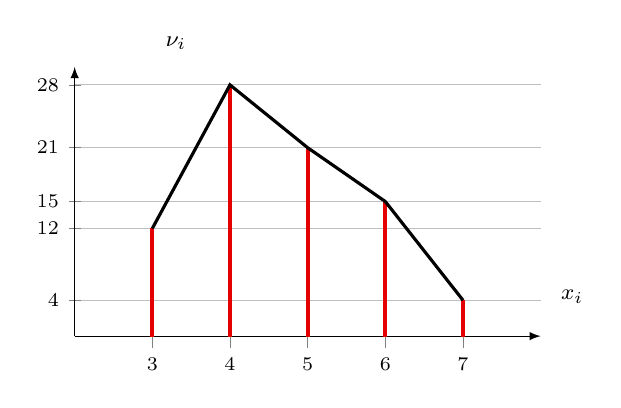
\begin{tikzpicture}
\begin{axis}[axis lines=left,belh ar,ybar,enlarge x limits=0.25,bar width=1pt,ymin=0,ylabel={\footnotesize \rotatebox{-90}{$ \nu_i $}},xlabel={\footnotesize $ x_i $},xlabel style={at={(current axis.right of origin)},xshift=4mm,yshift=5mm, anchor=center},ylabel style={at={(current axis.above origin)},xshift=3mm,yshift=-3mm,,anchor=center},
height=5cm,width=7.5cm,symbolic x coords={$ 3 $,$ 4 $,$ 5 $,$ 6 $,$ 7 $},
xtick = data,ymajorticks=true,ymajorgrids = true,
ytick={4,12,15,21,28},
yticklabels= {4,12,15,21,28},ymax=30]
\addplot
[draw=red!90!black,fill=red!90!black] 
coordinates
{($ 3 $,12) ($ 4 $,28) ($ 5 $,21) ($ 6 $,15) ($ 7 $,4)};
\draw[plm](axis cs:{$ 3 $},12) -- (axis cs:{$ 4 $},28) -- (axis cs:{$ 5 $},21) -- (axis cs:{$ 6 $},15) -- (axis cs:{$ 7 $},4);
\end{axis}
\end{tikzpicture}\quad
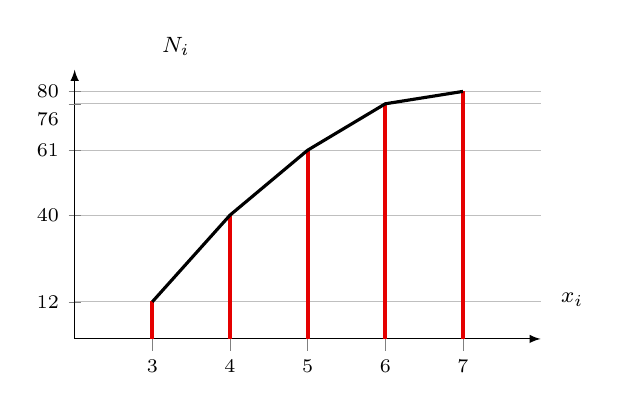
\begin{tikzpicture}
\begin{axis}[axis lines=left,belh ar,ybar,enlarge x limits=0.25,bar width=1pt,ymin=0,ylabel={\footnotesize \rotatebox{-90}{$ N_i $}},xlabel={\footnotesize $ x_i $},xlabel style={at={(current axis.right of origin)},xshift=4mm,yshift=5mm, anchor=center},ylabel style={at={(current axis.above origin)},xshift=3mm,yshift=-3mm,anchor=center},
height=5cm,width=7.5cm,symbolic x coords={$ 3 $,$ 4 $,$ 5 $,$ 6 $,$ 7 $},
xtick = data,ymajorticks=true,ymajorgrids = true,
ytick={12,40,61,80},
yticklabels= {12,40,61,80},ymax=87
,extra y ticks={76}
,extra y tick labels={76},
    extra y tick style={tick label style={yshift=-2mm}}]
\addplot
[draw=red!90!black,fill=red!90!black] 
coordinates
{($ 3 $,12) ($ 4 $,40) ($ 5 $,61) ($ 6 $,76) ($ 7 $,80)};
\draw[plm](axis cs:{$ 3 $},12) -- (axis cs:{$ 4 $},40) -- (axis cs:{$ 5 $},61) -- (axis cs:{$ 6 $},76) -- (axis cs:{$ 7 $},80);
\end{axis}
\end{tikzpicture}
\end{center}
\Paradeigma{Κυκλικό διάγραμμα}
\wrapr{-5mm}{9}{3.5cm}{-5mm}{\begin{mytblr}{columns = {8mm,c},column{1} = {18mm,c},row{1}={m},row{odd} = {ht=4mm},
 row{even} = {ht=4mm},}
{Μάρκα \bmath{$x_i$}} & \bmath{$\nu_i$}\\
\eng{Fiat} & 20\\ \eng{Peugeot} & 35\\ \eng{Kia} & 40\\ \eng{Opel} & 25\\ 
\textbf{Σύνολο} & \bmath{$120$ }
\end{mytblr}}{
\bmath{Εξετάσαμε ένα δείγμα $120$ οικογενειών ως προς τη μάρκα αυτοκινήτου που οδηγούν και τα αποτελέσματα φαίνονται στο διπλανό πίνακα. Να κατασκευάσετε κυκλικό διάγραμμα συχνοτήτων για τα δεδομένα αυτά.}\\
\lysh
Με τη βοήθεια του τύπου $a_i=\frac{\nu_i}{\nu}\cdot360\degree$ θα υπολογίσουμε το μέτρο κάθε τομέα του κυκλικού διαγράμματος. Έχουμε λοιπόν:
\begin{multicols}{2}
\begin{itemize}
\item $a_1=\frac{\nu_1}{\nu}\cdot 360\degree=\frac{20}{120}\cdot360\degree=60\degree$
\item $a_2=\frac{\nu_2}{\nu}\cdot 360\degree=\frac{35}{120}\cdot360\degree=105\degree$
\item $a_3=\frac{\nu_3}{\nu}\cdot 360\degree=\frac{40}{120}\cdot360\degree=120\degree$
\item $a_4=\frac{\nu_4}{\nu}\cdot 360\degree=\frac{25}{120}\cdot360\degree=75\degree$
\end{itemize}
\end{multicols}
\wrapl{0mm}{6}{7cm}{-15mm}{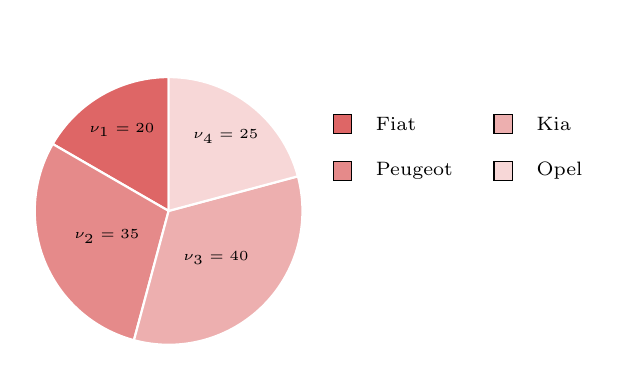
\begin{tikzpicture}
[pie chart,slice type={Fiat}{red6},
slice type={Peugeot}{red7},
slice type={Kia}{red8},
slice type={Opel}{red9},
pie values/.style={font={\tiny }},
scale=1.7
]
\pie[values of Fiat/.style={pos=.7},values of Opel/.style={pos=.7}]{}{20/Fiat/\nu_1=20,35/Peugeot/\nu_2=35,40/Kia/\nu_3=40,25/Opel/\nu_4=25}{120}
\eng
\legend[shift={(1.3cm,1cm)}]{{Fiat}/Fiat, {Peugeot}/Peugeot}
\legend[shift={(2.5cm,1cm)}]{{Kia}/Kia, {Opel}/Opel}
\gr
\end{tikzpicture}}{
Στη συνέχεια κατασκευάζουμε κύκλο στον οποίο φέρουμε μια ακτίνα ως πλευρά της 1ης γωνίας και σχεδιάζουμε γωνία $60\degree$. Συνεχίζουμε διαδοχικά για τις γωνίες $105\degree,120\degree$ και $75\degree$. Η τελική πλευρά κάθε γωνίας είναι αρχή της επόμενης. Όταν σχεδιαστεί και η προτελευταία γωνία, τότε προκύπτει αυτομάτως και η τελευταία που συμπληρώνει τον κύκλο.}\\\\\\
}
\Paradeigma{Ιστόγραμμα συχνοτήτων}
\bmath{Κατασκευάστε ιστόγραμμα και πολύγωνο συχνοτήτων καθώς και αθροιστικών συχνοττηων επί τοις \%, για τα δεδομένα του παραδείγματος \ref{Parad:Omadopoihsh}}\\
\lysh
Για το μεν ιστόγραμμα συχνοτήτων θα προσθέσουμε δύο επιπλέον κλάσεις, μια πριν την πρώτη και μια μετά την τελευταία στον οριζόντιο άξονα. Αφού κατασκευαστεί το ιστόγραμμα, ενώνουμε με τμήματα τα μέσα των άνω πλευρών κάθε ορθογωνίου. Για το δε πολύγωνο αθροιστικών σχετικών συχνοτήτων επί τοις $\%$, ενώνουμε τα άνω δεξιά άκρα, χωρίς την προσθήκη των επιπλέον κλάσεων.
\begin{center}
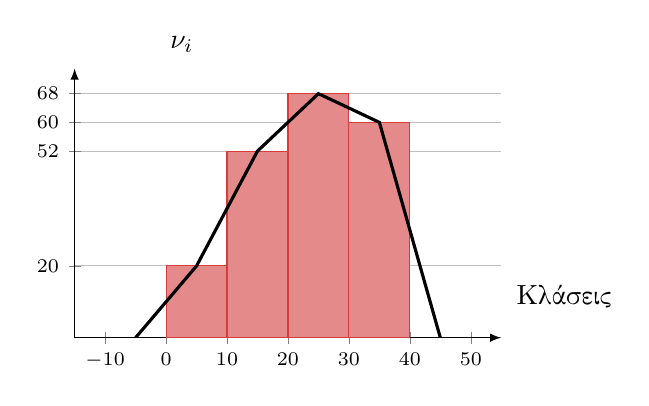
\begin{tikzpicture}
\begin{axis}[axis lines=left,belh ar,width=7cm,
height=5cm,xmin=-15,xmax=55,xlabel style={at={(current axis.right of origin)},xshift=8mm,yshift=5mm, anchor=center},
ylabel style={at={(current axis.above origin)},xshift=3mm,yshift=-2mm,anchor=center},
ymin=0, ymax=75,xlabel={Κλάσεις},ylabel={\rotatebox{-90}{$ \nu_i $}},xtick={-10,0,10,20,30,40,50},
xticklabels={$-10$,$0$,$10$,$20$,$30$,$40$,$50$},ymajorticks=true,ymajorgrids=true,ytick={20,52,60,68},
yticklabels= {20,52,60,68}]
\draw[color=red5,fill=red7] (axis cs:0,0) rectangle (axis cs:10,20);
\draw[color=red5,fill=red7] (axis cs:10,0) rectangle (axis cs:20,52);
\draw[color=red5,fill=red7] (axis cs:20,0) rectangle (axis cs:30,68);
\draw[color=red5,fill=red7] (axis cs:30,0) rectangle (axis cs:40,60);
\draw[plm] (axis cs:-5,0)--(axis cs:5,20)--(axis cs:15,52)--(axis cs:25,68)--(axis cs:35,60)--(axis cs:45,0);
\end{axis}
\end{tikzpicture}\quad
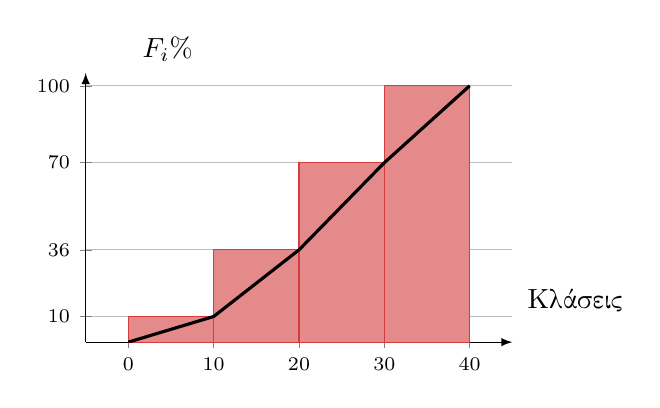
\begin{tikzpicture}
\begin{axis}[axis lines=left,belh ar,width=7cm,
height=5cm,xmin=-5,xmax=45,xlabel style={at={(current axis.right of origin)},xshift=8mm,yshift=5mm, anchor=center},
ylabel style={at={(current axis.above origin)},xshift=3mm,yshift=-5mm,anchor=center},
ymin=0, ymax=105,xlabel={Κλάσεις},ylabel={\rotatebox{-90}{$F_i\%$}},xtick={0,10,20,30,40}, xticklabels={$0$,$10$,$20$,$30$,$40$},ymajorticks=true,ymajorgrids=true,ytick={10,36,70,100},
yticklabels= {10,36,70,100}]
\draw[color=red5,fill=red7] (axis cs:0,0) rectangle (axis cs:10,10);
\draw[color=red5,fill=red7] (axis cs:10,0) rectangle (axis cs:20,36);
\draw[color=red5,fill=red7] (axis cs:20,0) rectangle (axis cs:30,70);
\draw[color=red5,fill=red7] (axis cs:30,0) rectangle (axis cs:40,100);
\draw[plm] (axis cs:0,0)--(axis cs:10,10)--(axis cs:20,36)--(axis cs:30,70)--(axis cs:40,100);
\end{axis}
\end{tikzpicture}
\end{center}
\begin{askhsh}{Μέσος όρος - Σταθμικός μέσος}
\begin{itemize}
\item Χρησιμοποιούμε τους τύπους \ref{meshtimh} για το μέσο όρο, ανάλογα με το αν η άσκηση μας δίνει παρατηρήσεις $t_i$, συχνότητες $\nu_i$ ή σχετικές συχνότητες $f_i$.
\item Για το σταθμικό μέσο χρησιμοποιείται ο τύπος \ref{stahmikos}.
\end{itemize}
\end{askhsh}
\Paradeigma{Μέση τιμή από δείγμα παρατηρήσεων}
\bmath{Οι μισθοί $10$ υπαλλήλων μιας εταιρίας είναι οι ακόλουθοι
\begin{gather*}
 1.020\euro,1.100\euro,980\euro,1.020\euro,1.200\euro,990\euro,1.070\euro,950\euro,1.080\euro,1.130\euro
\end{gather*}
Να βρείτε το μέσο μισθό των υπαλλήλων.}\\
\noindent
\lysh
Ο μέσος όρος των μισθών των $10$ υπαλλήλων θα είναι
\begin{align*}
 \bar{x}&=\frac{1}{\nu}\sum_{i=1}^{\nu}{t_i}=\\&=\frac{1.020+1.100+980+1.020+1.200+990+1.070+950+1.080+1.130}{10}=\frac{10.540}{10}=1.054\euro
\end{align*}
\Paradeigma{Μέση τιμή από πίνακα συχνοτήτων $\nu_i$}\label{padadeigma:diamesos_Ni}
\wrapr{-5mm}{4}{4cm}{-10mm}{\begin{mytblr}{columns = {8mm,c},column{1} = {18mm,c},row{1}={m},row{odd} = {ht=4mm},
 row{even} = {ht=4mm},}
{Χρόνος \bmath{$x_i$}} & \bmath{$\nu_i$}\\
3 & 28\\ 4 & 32\\ 5 & 12\\ 6 & 8\\
Σύνολο & $80$ 
\end{mytblr}}{\bmath{Στον διπλανό πίνακα βλεπουμε την κατανομή συχνοτήτων ενός δείγματος $80$ ατόμων για το χρόνο παρακολούθησης τηλεόρασης καθημαρινά. Να υπολογίσετε το μέσο χρόνο παρακολούθησης.}\\
\lysh
Υπολογίζουμε τα γινόμενα $x_i\cdot\nu_i$ για κάθε $i=1,2,\ldots,\kappa$.
\begin{multicols}{2}
\begin{itemize}
\item $x_1\cdot \nu_1=3\cdot28=84$
\item $x_2\cdot \nu_2=4\cdot32=128$
\item $x_3\cdot \nu_3=5\cdot12=60$
\item $x_4\cdot \nu_4=6\cdot8=48$
\end{itemize}
\end{multicols}
Θα έχουμε λοιπόν \[ \bar{x}=\frac{1}{\nu}{\sum_{i=1}^{\kappa}{x_i\cdot\nu_i}}=\frac{84+128+60+48}{80}=\frac{320}{80}=4\textrm{ ώρες} \]
}
\Paradeigma{Μέση τιμή από πίνακα συχνοτήτων $f_i$}\label{padadeigma:diamesos_Fi}
\wrapr{-5mm}{10}{4cm}{-10mm}{\begin{mytblr}{columns = {8mm,c},column{1} = {18mm,c},row{1}={m},row{odd} = {ht=4mm},
 row{even} = {ht=4mm},}
{Χρόνος \bmath{$x_i$}} & \bmath{$f_i$}\\
$7$ & $0{,}22$\\ $8$ & $0{,}36$\\ $9$ & $0{,}3$\\ $10$ & $0{,}12$\\
Σύνολο & $1$ 
\end{mytblr}}{\bmath{Ο διπλανός πίνακας περιέχει την κατανομή σχετικών συχνοτήτων ενός δείγματος $50$ αθλητών ως προς τις ώρες που αθλούνται εβδομαδιαίως. Υπολογίστε το μέσο χρόνο προπόνησης κάθε αθλητή.}\\
\lysh
Υπολογίζουμε τα γινόμενα $x_i\cdot f_i$ για κάθε $i=1,2,\ldots,\kappa$.
\begin{multicols}{2}
\begin{itemize}
\item $x_1\cdot f_1=7\cdot0{,}22=1{,}54$
\item $x_2\cdot f_2=8\cdot0{,}36=2{,}88$
\item $x_3\cdot f_3=9\cdot0{,}3=2{,}7$
\item $x_4\cdot f_4=10\cdot0{,}12=1{,}2$
\end{itemize}
\end{multicols}
Θα έχουμε λοιπόν \[ \bar{x}=\sum_{i=1}^{\kappa}{x_i\cdot f_i}=1{,}54+2{,}88+2{,}7+1{,}2=8{,}32\textrm{ ώρες} \]
}
\Paradeigma{Σταθμικός μέσος}
\bmath{Τα τέσσερα μαθήματα Α,Β,Γ,Δ στο 1ο εξάμηνο μιας σχολής έχουν συντελεστές βαρύτητας $2,3,1{.}5$ και $2{.}5$ αντίστοιχα. Οι βαθμοί ενος φοιτητή στα μαθήματα αυτά είναι $7,8,10,9$. Να υπολογίσετε το μέσο όρο του για το 1ο εξάμηνο.}\\
\lysh
Κάθε βαθμός θα πολλαπλασιαστεί με τον αντίστοιχο συντελεστή βαρύτητας. Έτσι ο σταθμικός μέσος θα είναι:
\[ \bar{x}=\frac{\sum_{i=1}^{\kappa}{x_i\cdot w_i}}{\sum_{i=1}^{\kappa}{w_i}}=\frac{2\cdot 7+3\cdot8+1.5\cdot 10+2.5\cdot 9}{2+3+1.5+2.5}=\frac{75.5}{9}=8.38 \]
\begin{askhsh}{Υπολογισμός διαμέσου από παρατηρήσεις $t_i$}
\begin{itemize}
\item Αν το πλήθος $\nu$ των παρατηρήσεων είναι \textbf{περιττό}, τότε η διάμεσος ισούται με τη μεσαία παρατήρηση. Δηλαδή
\[ \delta=t_{\frac{\nu+1}{2}} \]
\item Αν το πλήθος $\nu$ των παρατηρήσεων είναι \textbf{άρτιο}, τότε η διάμεσος ισούται με το ημιάθροισμα των δύο μεσαίων παρατηρήσεων. Δηλαδή
\[ \delta=\frac{t_{\frac{\nu}{2}}+t_{\frac{\nu}{2}+1}}{2} \]
\end{itemize}
\end{askhsh}
\noindent
\Paradeigma{Διάμεσος από δείγμα παρατηρήσεων}
\bmath{Να υπολογίσετε τη διάμεσο σε καθένα από τα παρακάτω δείγματα.
\begin{alist}
\item $12,10,9,11,8,13,10,12,12$
\item $8,5,6,9,4,3,3,5,6,7$
\end{alist}}
\noindent
\lysh\vspace{-7mm}
\begin{alist}
\item Οι παρατηρήσεις σε αύξουσα σειρά είναι :
\[8,9,10,10,11,12,12,12,13\]
Το πλήθος τους είναι $\nu=9$ δηλαδή περιττό. Η μεσαία παρατήρηση βρίσκεται στη θέση $\frac{\nu+1}{2}=\frac{10}{2}=5$ άρα η διάμεσος θα ισούται με την 5η παρατήρηση : $\delta=t_5=11$.
\item Τοποθετούμε αρχικά τις παρατηρήσεις σε αύξουσα σειρά :
\[3,3,4,5,5,6,6,7,8,9\]
Το πλήθος των παρατηρήσεων είναι $\nu=10$ δηλαδή άρτιο. Έτσι οι δύο μεσαίες παρατηρήσεις βρίσκονται στις θέσεις
\[ \frac{\nu}{2}=\frac{10}{2}=5\textrm{ και }\frac{\nu+2}{2}=\frac{12}{2}=6 \]
Άρα η διάμεσος θα ισούται με 
\[\delta=\frac{t_5+t_6}{2}=\frac{5+6}{2}=\frac{11}{2}=5{,}5\]

\end{alist}
\begin{askhsh}{Υπολογισμός διαμέσου από συχνότητες $N_i$}\label{diamesos1}
Υπολογίζουμε τις αθροιστικές συχνότητες $N_i$ καθώς και το \textbf{μισό μέγεθος του δείγματος}, δηλαδή το $\frac{\nu}{2}$.
\begin{itemize}[leftmargin=4mm]
\item Αν το πλήθος είναι \textbf{περιττό}, η διάμεσος είναι η τιμή $x_i$ στην οποία η $N_i$ \textbf{ξεπερνάει πρώτη φορά} το $\frac{\nu}{2}$.
\item Αν το πλήθος είναι \textbf{άρτιο}, τότε στη στήλη $N_i$ εξετάζουμε τις εξής περιπτώσεις:
\begin{itemize}
\item Αν εμφανίζεται σε κάποια γραμμή $i$ το $\frac{\nu}{2}$, τότε η διάμεσος ισούται με 
\[ \delta=\frac{x_i+x_{i+1}}{2} \]
\item Αν \textbf{δεν} εμφανίζεται σε κάποια γραμμή $i$ το $\frac{\nu}{2}$, τότε η διάμεσος ισούται με την τιμή $x_i$ στην οποία η $N_i$ \textbf{ξεπερνάει πρώτη φορά} τον αριθμό αυτό.
\end{itemize}
\end{itemize}
\end{askhsh}
\Paradeigma{Διάμεσος με τη χρήση $N_i$}
\bmath{Χρησιμοποιώντας τα δεδομένα από το παράδειγμα \ref{padadeigma:diamesos_Ni} να υπολογίστεί η διάμεσος του δείγματος.}\\
\lysh
\wrapr{-5mm}{5}{4.8cm}{-5mm}{
\begin{mytblr}{columns = {8mm,c},column{1} = {18mm,c},row{1}={m},row{odd} = {ht=4mm},
 row{even} = {ht=4mm},}
{Χρόνος \bmath{$x_i$}} & \bmath{$\nu_i$} & \bmath{$N_i$}\\
3 & 28 & 28\\ 4 & 32 & 60\\ 5 & 12 & 72\\ 6 & 8 & 80\\
Σύνολο & $80$ & \SetCell{bg=gray7} 
\end{mytblr}}{
Υπολογίζουμε, με τη βοήθεια του πίνακα του παραδείγματος, τις αθροιστικές συχνότητες $N_i$:
\begin{itemize}
\item $N_1=\nu_1=28$
\item $N_2=N_1+\nu_2=28+32=60$
\item $N_3=N_2+\nu_3=60+12=72$
\item $N_4=\nu=80$
\end{itemize}}
Παρατηρούμε ότι στη στήλη των αθροιστικών συχνοτήτων, ξεπερνάμε πρώτη φορά το μισό δείγμα $\frac{\nu}{2}=\frac{80}{2}=40$ στη 2η γραμμή του πίνακα. Επομένως η διάμεσος θα ισούται με $\delta=x_2=4$ ώρες.
\begin{askhsh}{Υπολογισμός διαμέσου από συχνότητες $F_i\%$}\label{diamesos2}
Ακολουθούμε τα ίδια βήματα με την παραπάνω μέθοδο, χρησιμοποιώντας τη στήλη των αθροιστικών σχετικών συχνοτήτων $F_i\%$ και ως μισό δείγμα το $50\%$.
\end{askhsh}\mbox{}\\
\Paradeigma{Διάμεσος με τη χρήση $F_i$}
\bmath{Χρησιμοποιώντας τα δεδομένα από το παράδειγμα \ref{padadeigma:diamesos_Fi} να υπολογίστεί η διάμεσος του δείγματος.}\\
\lysh
\wrapr{-5mm}{5}{4.8cm}{-5mm}{
\begin{mytblr}{columns = {8mm,c},column{1} = {18mm,c},row{1}={m},row{odd} = {ht=4mm},
 row{even} = {ht=4mm},}
{Χρόνος \bmath{$x_i$}} & \bmath{$f_i$} & \bmath{$F_i\%$}\\
$7$ & $0{,}22$ & $22$\\ $8$ & $0{,}36$ & $58$\\ $9$ & $0{,}3$ & $88$\\ $10$ & $0{,}12$ & $100$\\
Σύνολο & $1$ & \SetCell{bg=gray7}
\end{mytblr}}{
Υπολογίζουμε, με τη βοήθεια του πίνακα, τις αθροιστικές σχετικές συχνότητες $F_i\%$:
\begin{itemize}
\item $F_1\%=f_1\%=0{,}22\cdot 100=22$
\item $F_2\%=F_1\%+f_2\%=22+0{,}36\cdot 100=22+36=58$
\item $F_3\%=F_2+f_3=58+0{,}3\cdot 100=88$
\item $F_4\%=100$
\end{itemize}
Παρατηρούμε ότι στη στήλη των αθροιστικών σχετικών συχνοτήτων, ξεπερνάμε πρώτη φορά το $50\%$ στη 2η γραμμή του πίνακα. Επομένως η διάμεσος θα ισούται με $\delta=x_2=8$ ώρες.}
\begin{askhsh}{Υπολογισμός εύρους}
Χρησιμοποιείται οι τύποι \ref{evros}.
\end{askhsh}\mbox{}\\
\Paradeigma{Υπολογισμός εύρους - Δείγμα παρατηρήσεων}
\bmath{Βρείτε το εύρος των παρατηρήσεων στο δείγμα που ακολουθεί
\[ 10,4,-2,8,7,5,-1.9,6,7 \]}
\lysh
Η μέγιστη παρατήρηση του δείγματος είναι $t_{\max}=10$ ενώ η ελάχιστη είναι $t_{\min}=-2$. Έτσι το εύρος ισούται με
\[ R=t_{\max}-t_{\min}=10-(-2)=12 \]
\Paradeigma{Υπολογισμός εύρους - Πίνακας συχνοτήτων}
\bmath{Υπολογίστε για τα παραδείγματα \ref{padadeigma:diamesos_Ni} και \ref{padadeigma:diamesos_Fi} το εύρος των παρατηρήσεων.}\\
\lysh 
Σύμφωνα με το παράδειγμα {\ref{padadeigma:diamesos_Ni}} οι μέγιστη και ελάχιστη τιμή είναι αντίστοιχα $x_{\max}=6$ και $x_{\min}=3$ οπότε το εύρος είναι $R=6-3=3$ ώρες. Ομοίως από το παράδειγμα {\ref{padadeigma:diamesos_Fi}} είναι $R=x_{\max}-x_{\min}=10-7=3$
\begin{askhsh}{Διακύμανση - Τυπική απόκλιση}
\begin{itemize}
\item Για τον υπολογισμό της διακύμανσης χρησιμοποιούμε τους τύπους \ref{diakymansh} ανάλογα με το ποια συχνότητα θα χρησιμοποιήσουμε αλλά και με το αν ο μέσος όρος $\bar{x}$ είναι ακέραιος ή όχι.
\item Για τον υπολογισμό της τυπικής απόκλισης $s$ χρησιμοποιούμε τον τύπο $s=\sqrt{s^2}$.
\end{itemize}
\end{askhsh}
\noindent\Paradeigma{Διακύμανση - τυπική απόκλιση από παρατηρήσεις}
\bmath{Να βρεθεί η διακύμανση και η τυπική απόκλιση στα παρακάτω δείγματα παρατηρήσεων
\begin{alist}
\item $A: 1,4,5,5,7,8$
\item $B: 2,3,4,4,5,6,8,8,9$
\end{alist}}
\noindent\lysh
Υπολογίζουμε αρχικά τη μέση τιμή για κάθε δείγμα.
\begin{alist}
\item Για το δείγμα Α έχουμε
\[ \bar{x}_A=\frac{1}{\nu}\sum_{i=1}^{\nu}=\frac{1+4+5+5+7+8}{6}=\frac{30}{6}=5 \]
Καθώς η μέση τιμή είναι ακέραια, η διακύμανση του δείγματος θα είναι
\begin{align*}
s^2&=\frac{1}{\nu}\sum_{i=1}^{\nu}{(t_i-\bar{x})}=\\
&=\frac{(1-5)^2+(4-5)^2+(5-5)^2+(5-5)^2+(7-5)^2+(8-5)^2}{6}=\\&=\frac{(-4)^2+(-1)^2+0^2+0^2+2^2+3^2}{6}=\frac{16+1+4+9}{6}=\frac{30}{6}=5
\end{align*}
Επίσης η τυπική απόκλιση θα ισούται με $s=\sqrt{s^2}=\sqrt{5}\simeq 2{,}236$.
\item Ομοίως για το δείγμα Β είναι:
\[ \bar{x}_B=\frac{1}{\nu}\sum_{i=1}^{\nu}=\frac{2+3+4+4+5+6+8+8+9}{9}=\frac{49}{9}=5{,}44 \]
Αφού η μέση τιμή δεν είναι ακέραια, τότε για τη διακύμανση του δείγματος θα έχουμε
\begin{itemize}
\item $\sum\limits_{i=1}^{\nu}{t_i^2}=2^2+3^2+4^2+4^2+5^2+6^2+8^2+8^2+9^2=315$
\item $\left( \sum\limits_{i=1}^{\nu}{t_i}\right)^2=49^2=2.401$
\end{itemize}
\[
s^2=\dfrac{1}{\nu}\LEFTRIGHT\{\}{\sum\limits_{i=1}^{\nu}{t_i^2}-\frac{\left( \sum\limits_{i=1}^{\nu}{t_i}\right)^2 }{\nu}}=\frac{1}{9}\left(315-\frac{2.401}{9}\right)=\frac{1}{9}\left(315-266{,}77\right)=\frac{48{,}23}{9}=5{,}35
\]
Άρα η τυπική απόκλιση θα είναι $s=\sqrt{s^2}=\sqrt{5{,}358}=2{,}315$
\end{alist}
\Paradeigma{Διακύμανση - τυπική απόκλιση από συχνότητες $\nu_i$}
\bmath{Επιλέξαμε δύο δείγματα $50$ μαθητών Γ' ΕΠΑ.Λ. από δύο λύκεια της Αθήνας, τα οποία εξετάσαμε ως προς τη βαθμολογία στο διαγώνισμα Μαθηματικών στις πανελλαδικές. Τα αποτελέσματα φαίνονται στους παρακάτω πίνακες:
\begin{center}
\begin{tabular}{cc}
\begin{mytblr}{columns = {8mm,c},column{1} = {18mm,c},row{1}={m},row{odd} = {ht=4mm},
 row{even} = {ht=4mm},}
{Βαθμός \bmath{$x_i$}} & \bmath{$\nu_i$}\\
14 & 16\\ 15 & 22\\ 16 & 8 \\ 17 & 4 \\
Σύνολο & $50$
\end{mytblr} & \begin{mytblr}{columns = {8mm,c},column{1} = {18mm,c},row{1}={m},row{odd} = {ht=4mm},
 row{even} = {ht=4mm},}
{Βαθμός \bmath{$x_i$}} & \bmath{$\nu_i$}\\
14 & 9\\ 15 & 19\\ 16 & 15 \\ 17 & 7 \\
Σύνολο & $50$
\end{mytblr}
\end{tabular}
\end{center}
Να υπολογίσετε για κάθε δείγμα μαθητών τη διακύμανση και την τυπική απόκλιση των βαθμών.}\\
\lysh
Για το 1\tss{ο} δείγμα μαθητών υπολογίζουμε αρχικά το μέσο όρο των βαθμών τους. Έχουμε λοιπόν
\[ \bar{x}=\frac{1}{\nu}\sum_{i=1}^{\kappa}{x_i\cdot\nu_i}=\frac{14\cdot16+15\cdot22+16\cdot8+17\cdot4}{50}=\frac{750}{50}=15 \]
Η μέση τιμή είναι ακέραια οπότε για τη διακύμανση θα έχουμε
\begin{align*}
s^2&=\frac{1}{\nu}\sum_{i=1}^{\kappa}{(x_i-\bar{x})^2\cdot\nu_i}=\frac{(14-15)^2\cdot16+(15-15)^2\cdot22+(16-15)^2\cdot8+(17-15)^2\cdot4}{50}=\\
&=\frac{(-1)^2\cdot16+0^2\cdot22+1^2\cdot8+2^2\cdot4}{50}=\frac{40}{50}=0{,}8
\end{align*}
Επομένως η τυπική απόκλιση θα ισούται με $s=\sqrt{s^2}=\sqrt{0{,}8}=0{,}894$.\\ Για το δεύτερο δείγμα η μέση τιμή θα είναι
\[ \bar{x}=\frac{1}{\nu}\sum_{i=1}^{\kappa}{x_i\cdot\nu}=\frac{14\cdot9+15\cdot19+16\cdot15+17\cdot7}{50}=\frac{770}{50}=15{,}4 \]
Μιας και η μέση τιμή δεν είναι ακέραια, για τη διακύμανση θα έχουμε
\begin{itemize}
\item $\sum\limits_{i=1}^{\kappa}{x_i^2\cdot\nu_i}=14^2\cdot9+15^2\cdot19+16^2\cdot15+17^2\cdot7=11.902$
\item $\left( \sum\limits_{i=1}^{\kappa}{x_i\cdot\nu_i}\right)^2=770^2=592.900$
\end{itemize}
\[
s^2=\dfrac{1}{\nu}\LEFTRIGHT\{\}{\sum\limits_{i=1}^{\kappa}{x_i^2\cdot\nu_i}-\frac{\left( \sum\limits_{i=1}^{\kappa}{{x_i\cdot\nu_i}}\right)^2 }{\nu}}=\frac{1}{50}\left(11.902-\frac{592.900}{50}\right)=\frac{1}{50}\left(11.902-11.858\right)=\frac{44}{50}=0{,}98
\]
Άρα η τυπική απόκλιση θα είναι $s=\sqrt{s^2}=\sqrt{0{,}98}=0{,}99$.\\
\Paradeigma{Διακύμανση - τυπική απόκλιση από συχνότητες $f_i$}
\bmath{Χρησιμοποιώντας τα δεδομένα από το παράδειγμα \ref{padadeigma:diamesos_Fi} να υπολογίστεί η διακύμανση και η τυπική απόκλιση του δείγματος.}\\
\lysh
Έχουμε βρει από το παράδειγμα ότι $\bar{x}=8{,}32$. Για τη διακύμανση είναι
\begin{align*}
s^2&=\displaystyle\sum\limits_{i=1}^{\kappa}{x_i^2f_i-(\bar{x})^2}=\\
&=7^2\cdot0{,}22+8^2\cdot0{,}36+9^2\cdot0{,}3+10^2\cdot0{,}12-8{,}32^2=\\
&=10{,}78+23{,}04+24{,}3+12=70{,}12-69{,}22=0{,}9
\end{align*}
άρα η τυπική απόκλιση ισούται με $s=\sqrt{s^2}=\sqrt{0{,}9}=0{,}949$.
\begin{askhsh}{Υπολογισμός συντελεστή μεταβολής}
\begin{alist}
\item Υπολογίζουμε μέση τιμή $\bar{x}$ και τυπική απόκλιση $s$.
\item Χρησιμοποιούμε τον τύπο $CV=\dfrac{s}{|\bar{x}|}$ και εκφράζουμε το αποτέλεσμα ως ποσοστό $\%$.
\end{alist}
\begin{itemize}
\item Αν $CV>10\%$ το δείγμα δεν είναι ομοιογενές. Αν $CV\leq 10\%$ το δείγμα είναι ομοιογενές.
\item Αν για δύο δείγματα ισχύει $CV_A>CV_B$ το δείγμα $B$ είναι πιο ομοιογενές από το $A$.
\end{itemize}
\end{askhsh}
\noindent
\Paradeigma{Συντελεστής μεταβολής - Ομοιογένεια}
\bmath{Οι βαθμοί δύο μαθητών στα $10$ μαθήματα του Α' τετραμήνου δίνονται παρακάτω.\\\\
\begin{minipage}{0.5\textwidth}
\begin{center}
Μαθητής Α
\begin{gather*}
15,16,15,17,16,\\15,14,17,15,16
\end{gather*}
\end{center}
\end{minipage}\hfill
\begin{minipage}{0.5\textwidth}
\begin{center}
Μαθητής Β
\begin{gather*}
12,18,17,17,18,\\19,10,12,20,13
\end{gather*}
\end{center}
\end{minipage}
\begin{alist}
\item Να εξετάσετε κάθε δείγμα ως προς την ομοιογένεια.
\item Ποιο από τα δύο δείγματα είναι πιο ομοιογενές?
\end{alist}}
\noindent\lysh\vspace{-5mm}
\begin{alist}
\item Υπολογίζουμε αρχικά το μέσο όρο των μαθημάτων του για το μαθητή Α:
\[ \bar{x}=\frac{1}{\nu}\sum_{i=1}^{\nu}{t_i}=\frac{15+16+15+17+16+15+14+17+15+16}{10}=\frac{156}{10}=15{,}6 \]
Καθώς η μέση τιμή δεν είναι ακέραια τότε για την διακύμανση έχουμε:
\begin{itemize}
\item $\sum\limits_{i=1}^{\nu}{t_i^2}=15^2+16^2+15^2+17^2+16^2+15^2+14^2+17^2+15^2+16^2=2442$
\item $\left( \sum\limits_{i=1}^{\nu}{t_i}\right)^2=156^2=24.336$
\end{itemize}
\[
s^2=\dfrac{1}{\nu}\LEFTRIGHT\{\}{\sum\limits_{i=1}^{\nu}{t_i^2}-\frac{\left( \sum\limits_{i=1}^{\nu}{t_i}\right)^2 }{\nu}}=\frac{1}{10}\left(2.442-\frac{24.336}{10}\right)=\frac{1}{10}\left(2.442-2433{,}6\right)=\frac{8{,}4}{10}=0{,}84
\]
Έτσι η τυπική απόκλιση θα ισούται με $s=\sqrt{s^2}=\sqrt{0{,}84}=0{,}9165$. Ο συντελεστής μεταβλητότητας του μαθητή θα είναι
\[ CV_A=\frac{s}{|\bar{x}|}=\frac{0{,}9156}{15{,}6}=0{,}06=6\%<10\% \]
Καταλήγουμε έτσι στο συμπέρασμα ότι το δείγμα των βαθμών για το μαθητή Α είναι ομοιογενές. Ομοίως για το μαθητή Β έχουμε
\[ \bar{x}=15{,}6\ ,\ s=3{,}5 \]
άρα ο συντελεστής μεταβολής θα είναι
\[ CV_B=\frac{s}{|\bar{x}|}=\frac{3{,}5}{15{,}6}=0{,}2243=22{,}43\%>10\% \]
Το δεύτερο δείγμα δεν είναι ομοιογενές.
\item Σύμφωνα με τα προηγούμενα βλέπουμε $CV_A<CV_B$ άρα το 1\tss{ο} δείγμα έχει μεγαλύτερη ομοιογένεια.
\end{alist}
\begin{askhsh}{Κανονική κατανομή}
\begin{alist}
\item Σχεδιάζουμε την καμπύλη της κανονικής κατανομής και τοποθετούμε στον οριζόντιο άξονα τους κατάλληλους αριθμούς, αν γνωρίζουμε τα ποσά $\bar{x}$ και $s$.
\item Χρησιμοποιούμε τα ποσοστά που περιέχει κάθε περιοχή της καμπύλης για να απαντήσουμε σε ερωτήσεις ή να υπολογίσουμε πλήθος παρατηρήσεων με τον τύπο
\[ \textrm{Ποσοστό}=\frac{\textrm{Μέρος}}{\textrm{Ολόκληρο}nu_i}{\nu} \]
\item Αν μας ενδιαφέρουν πολλές περιοχές του σχήματος προσθέτουμε τα αντίστοιχα ποσοστά.
\end{alist}
\end{askhsh}
\Paradeigma{Κανονική κατανομή}
\bmath{Ο χρόνος (σε λεπτά) που χρησιμοποιούν οι πελάτες μιας εταιρίας το κινητό τους τηλέφωνο, ακολουθεί κανονική κατανομή. Γνωρίζουμε ότι το $84\%$ των πελατών χρησιμοποιεί το κινητό το πολύ $110$ λεπτά, ενώ το $99{,}85\%$ των πελατών το χρησιμοποιεί τουλάχιστον $70$ λεπτά.
\begin{alist}
\item Να δείξετε ότι $\bar{x}=100$ και $s=10$.
\item Να βρεθεί το ποσοστό των πελατών που μίλησαν
\begin{enumerate}[label=\roman*.]
\item τουλάχιστον $90$ λεπτά.
\item το πολύ $80$ λεπτά.
\item από $80$ έως $120$ λεπτά.
\end{enumerate}
\item Αν το σύνολο των πελατών είναι $\nu=4.000$ άτομα, να βρεθεί πόσοι πελάτες χρησιμοποίησαν το κινητό τουλάχιστον $110$ λεπτά.
\end{alist}}
\lysh\vspace{-7mm}
\begin{alist}
\item Κατασκευάζουμε αρχικά την καμπύλη της κανονικής κατανομής, τοποθετώντας πάνω στο άξονα τις τιμές από $\bar{x}-3s$ έως $\bar{x}+3s$. Από τη φράση \textbf{το πολύ} $110$ λεπτά καταλαβαίνουμε ότι πρέπει να προστεθούν τα ποσοστά έως και τη θέση $\bar{x}+s$ ώστε να πάρουμε το αντίστοιχο ποσοστό $84\%$. Άρα πρέπει $\bar{x}+s=110$.
\begin{center}
\begin{tikzpicture}
\begin{axis}[axis y line=none,aks_on,belh ar,
no markers,xmax=8, samples=200,
axis lines*=left, xlabel=$x_i$, ylabel=$\nu_i$,
every axis y label/.style={at=(current axis.above origin),anchor=south},ymin=0,
every axis x label/.style={at=(current axis.right of origin),anchor=west},
height=4.5cm, width=12cm,xticklabels={$ \bar{x}-3s $,$ \bar{x}-2s $,$ \bar{x}-s $,$ \bar{x} $,$ \bar{x}+s $,$ \bar{x}+2s $,$ \bar{x}+3s $},  xtick={1,2,3,4,5,6,7},enlargelimits=false, clip=false, axis on top]
\addplot [thick,fill=red!10,domain=0:1] {gauss(4,1)+0.015} \closedcycle;\addplot [fill=red!30, domain=1:2] {gauss(4,1)+0.015} \closedcycle;
\addplot [fill=red!10, domain=2:3] {gauss(4,1)+0.015} \closedcycle;
\addplot [fill=red!30, domain=3:4] {gauss(4,1)+0.015} \closedcycle;
\addplot [fill=red!30, domain=4:5] {gauss(4,1)+0.015} \closedcycle;
\addplot [fill=red!10, domain=5:6] {gauss(4,1)+0.015} \closedcycle;
\addplot [fill=red!30, domain=6:7] {gauss(4,1)+0.015} \closedcycle;
\addplot [fill=red!10, domain=7:8] {gauss(4,1)+0.015} \closedcycle;
\addplot [plm,draw=red!80!black,domain=0:8] {gauss(4,1)+0.015};
\node at (axis cs:3.5,0.15){\footnotesize$34\%$};
\node at (axis cs:4.5,0.15){\footnotesize$34\%$};
\node at (axis cs:5.5,0.05){\footnotesize$13{,}5\%$};
\node at (axis cs:6.5,0.08){\footnotesize$2{,}35\%$};
\node at (axis cs:7.5,0.08){\footnotesize$0{,}15\%$};
\node at (axis cs:2.5,0.05){\footnotesize$13{,}5\%$};
\node at (axis cs:1.5,0.08){\footnotesize$2{,}35\%$};
\node at (axis cs:0.5,0.08){\footnotesize$0{,}15\%$};
\draw[{Bar[]-latex[]}](axis cs:1,-.17)--(axis cs:8,-.17)node[pos=0.5,below] {$98{,}85\%$};
\draw[{latex[]-Bar[]}] (axis cs:0,-.13)--(axis cs:5,-.13)node[pos=0.5,above] {$84\%$};
\end{axis}
\end{tikzpicture}
\end{center}
Αντίστοιχα, από τη φράση \textbf{τουλάχιστον} $70$ λεπτά βλέπουμε ότι πρέπει να προστεθούν τα ποσοστά από τη θέση $\bar{x}-3s$ και μετά ώστε να προκύψει το ποσοστό $99{,}85\%$. Έτσι πρέπει $\bar{x}-3s=70$. Από αυτές τις δύο εξισώσεις προκύπτει το σύστημα:
\begin{gather*}
\syssubstitute{.,{a}{\bar{x}}{b}{s}}
\systeme{a+b=110,a-3b=70}\Rightarrow \bar{x}=70+3s\\
\textrm{Άρα }70+3s+s=110\Rightarrow4s=40\Rightarrow s=10\\
\textrm{και }x=70+3\cdot 10=100
\end{gather*}

\item Για $\bar{x}=100$ και $s=10$ συμπληρώνουμε τις τιμές στον οριζόντιο άξονα και τα ποσοστά σε κάθε τομέα μεταξύ της καμπύλης και του άξονα.
\begin{center}
\begin{tikzpicture}
\begin{axis}[axis y line=none,aks_on,belh ar,
no markers,xmax=8, samples=200,
axis lines*=left, xlabel=$x_i$, ylabel=$\nu_i$,
every axis y label/.style={at=(current axis.above origin),anchor=south},ymin=0,
every axis x label/.style={at=(current axis.right of origin),anchor=west},
height=4.5cm, width=12cm,xticklabels={$ 70 $,$ 80 $,$ 90 $,$ 100 $,$ 110 $,$ 120 $,$ 130 $},  xtick={1,2,3,4,5,6,7},enlargelimits=false, clip=false, axis on top]
\addplot [thick,fill=red!10,domain=0:1] {gauss(4,1)+0.015} \closedcycle;\addplot [fill=red!30, domain=1:2] {gauss(4,1)+0.015} \closedcycle;
\addplot [fill=red!10, domain=2:3] {gauss(4,1)+0.015} \closedcycle;
\addplot [fill=red!30, domain=3:4] {gauss(4,1)+0.015} \closedcycle;
\addplot [fill=red!30, domain=4:5] {gauss(4,1)+0.015} \closedcycle;
\addplot [fill=red!10, domain=5:6] {gauss(4,1)+0.015} \closedcycle;
\addplot [fill=red!30, domain=6:7] {gauss(4,1)+0.015} \closedcycle;
\addplot [fill=red!10, domain=7:8] {gauss(4,1)+0.015} \closedcycle;
\addplot [plm,draw=red!80!black,domain=0:8] {gauss(4,1)+0.015};
\node at (axis cs:3.5,0.15){\footnotesize$34\%$};
\node at (axis cs:4.5,0.15){\footnotesize$34\%$};
\node at (axis cs:5.5,0.05){\footnotesize$13{,}5\%$};
\node at (axis cs:6.5,0.08){\footnotesize$2{,}35\%$};
\node at (axis cs:7.5,0.08){\footnotesize$0{,}15\%$};
\node at (axis cs:2.5,0.05){\footnotesize$13{,}5\%$};
\node at (axis cs:1.5,0.08){\footnotesize$2{,}35\%$};
\node at (axis cs:0.5,0.08){\footnotesize$0{,}15\%$};
\end{axis}
\end{tikzpicture}
\end{center}
\begin{enumerate}[label*=\roman*.]
\item Για το μέρος των πελατών που μίλησαν τουλάχιστον $90$ λεπτά, βλέπουμε από το σχήμα τοι θα χρειαστούμε το κομμάτι της καμπύλης από το $90$ προς τα δεξιά. Έτσι το ζητούμενο ποσοστό είναι
\[ 34\%+34\%+13{,}5\%+2{,}35\%+0{,}15\%=84\% \]
\item Για όσους μίλησαν το πολύ $80$ λεπτά, χρειαζόμαστε το τμήμα της καμπύλης έως το σημείο αυτό άρα το ποσοστό θα είναι
\[ 0{,}15\%+2{,}35\%=2{,}5\% \]
\item Ομοίως με προηγουμένως το ζητούμενο ποσοστό θα είναι
\[ 13{,}5\%+34\%+34\%+13{,}5\%=95\% \]
\end{enumerate}
\item Έστω $x$ το πλήθος των πελατών που χρησιμοποίησαν το κινητό τουλάχιστον $110$ λεπτά. Το αντίστοιχο ποσοστό είναι:
\[ 13{,}5\%+2{,}35\%+0{,}15\%=16\% \]
Έτσι θα έχουμε
\begin{gather*}
16\%=\frac{x}{\nu}\Rightarrow\frac{16}{100}=\frac{x}{4000}\Rightarrow\\
100x=64000\Rightarrow x=640\ \textrm{πελατες.}
\end{gather*}
\end{alist}
\begin{askhsh}{Μεταβολές των παρατηρήσεων}
Αν οι τιμές $y_i$ μιας νέας μεταβλητής $Y$ προκύπτουν από πράξεις με τις τιμές $x_i$ της αρχικής μεταβλητής $X$, τότε χρησιμοποιούμε τον πίνακα \ref{pinakas3}.
\end{askhsh}
\noindent
\Paradeigma{Μεταβολές των παρατηρήσεων}\\
\bmath{Στο παρακάτω δείγμα βλέπουμε τις τιμές $10$ απορρυπαντικών σε ένα πολυκατάστημα
\[ 11\euro,7.8\euro,12.3\euro,9.4\euro,11.3\euro,8.9\euro,9.2\euro,7.9\euro,11.4\euro,10.8\euro \]
\begin{alist}
\item Υπολογίστε τη μέση τιμή και την τυπική απόκλιση του δείγματος.
\item Αν οι τιμές των προϊόντων αυξηθούν κατά $1.5\euro$ να εξετάσετε αν το δείγμα είναι ομοιογενές.
\item Το κατάστημα κάνει προσφορά $20\%$ στα απορρυπαντικά. Εξετάστε ανάμεσα στο αρχικό και στο τελικό δείγμα τιμών, ποιο έχει μεγαλύτερη ομοιογένεια.
\end{alist}}
\noindent\lysh\vspace{-7mm}
\begin{alist}
\item Η μέση τιμή των απορρυπαντικών ισούται με
\[ \bar{x}=\frac{1}{\nu}\sum_{i=1}^{\nu}{t_i}=\frac{11+7{,}8+12{,}3+9{,}4+11{,}3+8{,}9+9{,}2+7{,}9+11{,}4+10{,}8}{10}=\frac{100}{10}=10\euro \]
Εφόσον ο μέσος όρος είναι ακέραιος, η διακύμανση θα υπολογιστεί από τον 1ο τύπο στο \ref{diakymansh} και θα είναι 
\begin{multline*}
s^2=\frac{1}{\nu}\sum_{i=1}^{\nu}{(t_i-\bar{x})^2}=\frac{(11-10)^2+(7{,}8-10)^2+(12{,}3-10)^2+(9{,}4-10)^2+(11{,}3-10)^2+}{10}\\\frac{+(8{,}9-10)^2+(9{,}2-10)^2+(7{,}9-10)^2+(11{,}4-10)^2+(10{,}8-10)^2}{10}=
\end{multline*}
\[ =\frac{1^2+(-2{,}2)^2+2{,}3^2+(-0{,}6)^2+1{,}3^2+(-1{,}1)^2+(-0{,}8)^2+(-2{,}1)^2+1{,}4^2+0{,}8^2}{10}=\frac{22{,}04}{10}=2{,}204 \]
Άρα η τυπική απόκλιση είναι $s=\sqrt{s^2}=\sqrt{2{,}204}\simeq 1{,}485$.
\item Έστω $y_i,\ i=1,2,\ldots,10$ οι νέες τιμές των απορρυπαντικών που προκύπτουν από τις αρχικές τιμές $x_i$ με τι σχέση $y_i=x_i+1{,}5,\ i=1,2,\ldots,10$.
\begin{itemize}
\item Η νέα μέση τιμή θα έιναι $\bar{y}=\bar{x}+1{,}5=10+1{,}5=11{,}5\euro$.
\item Η νέα τυπική απόκλιση θα είναι $s_y=s_x=1{,}485\euro$.
\end{itemize}
Επομένως ο συντελεστής μεταβλητότητας του νέου δείγματος ισούται με
\[ CV_y=\frac{s_y}{|\bar{y}|}=\frac{1{,}485}{11{,}5}=0{,}129=12{,}9\%>10\% \]
Το δείγμα λοιπόν δεν είναι ομοιογενές.
\item  Έστω $z_i,\ i=1,2,\ldots,10$ οι νέες τιμές των απορρυπαντικών που προκύπτουν από τις αρχικές τιμές $x_i$ ύστερα από αύξηση κατά $20\%$ σύμφωνα με τη σχέση 
\[z_i=x_i+20\%x_i=x_i+0{,}2x_i=1{,}2x_i,\ i=1,2,\ldots,10\]
\begin{itemize}
\item Η νέα μέση τιμή θα είναι $\bar{z}=1{,}2\bar{x}=1{,}2\cdot 10=12\euro$.
\item Η νέα τυπική απόκλιση θα είναι $s_z=|1{,}2|s_x=1{,}2\cdot1{,}485=1{,}782\euro$.
\end{itemize}
Άρα ο νέος συντελεστής μεταβλητότητας θα είναι
\[ CV_z=\frac{s_z}{|\bar{z}|}=\frac{1{,}782}{12}=0{,}1485=14{,}85\% \]
Εφόσον $CV_y<CV_z$ τότε το προηγούμενο δείγμα έχει μεγαλύτερη ομοιογένεια.
\end{alist}
\Paradeigma{Μεταβολές των παρατηρήσεων - Συνδυαστικό θέμα}
\bmath{Δίνεται η συνάρτηση $f(x)=x^2+ax-2\ ,x\in\mathbb{R},\ a\in\mathbb{R}$ της οποίας η γραφική παράσταση διέρχεται από το σημείο $P(2,4)$.
\begin{alist}
\item Να δείξετε ότι $a=1$.
\item Να δείξετε ότι η εφαπτομένη της $C_f$ στο σημείο $A(-1,f(-1))$ έχει εξίσωση $y=-x-3$.
\item Έστω $A_i(x_i,y_i)\ ,\ i=1,2,\ldots100$, σημεία της εφαπτομένης της $C_f$ στο σημείο $A$. Αν γνωρίζουμε ότι οι τετμημένες $x_i$ των σημείων έχουν μέση τιμή $\bar{x}=4$ και τυπική απόκλιση $s_x=0{,}5$, να βρεθεί ο συντελεστής μεταβολής των τεταγμένων $y_i\ ,i=1,2,\ldots,100$ των σημείων.
\end{alist}}
\lysh\vspace{-5mm}
\begin{alist}
\item Αφού το σημείο $P(2,4)$ ανήκει στη γραφική παράσταση της $f$, τότε
\[ f(2)=4\Rightarrow2^2+a\cdot2-2=4\Rightarrow 2a=2\Rightarrow a=1 \]
\item Θέτοντας όπου $a=1$ ο τύπος της $f$ θα είναι $f(x)=x^2+x-2$. Για κάθε $x\in\mathbb{R}$ είναι
\[ f'(x)=(x^2+x-2)'=2x+1 \]
Αν $x=-1$ τότε:
\begin{itemize}
\item $f(-1)=(-1)^2-1-2=-2$ και 
\item $f'(-1)=2\cdot(-1)+1=-2+1=-1$.
\end{itemize}
Η εξίσωση της εφαπτομένης είναι
\[ y=\lambda x+\beta\Rightarrow y=-x+\beta \]
Αφού το σημείο $A(-1,-2)$ ανήκει στην ευθεία, τότε για $x=-1$ και $y=-2$ έχουμε:
\[ -2=-(-1)+\beta\Rightarrow \beta=-3 \]
άρα η ζητούμενη εφαπτομένη έχει εξίσωση $y=-x-3$.
\item Τα σημεία $A_i(x_i,y_i)$ είναι σημεία της εφαπτομένης του προηγούμενου ερωτήματος. Οι τεταγμένες τους λοιπόν θα δίνονται από τη σχέση
\[ y_i=-x_i-3\ ,\ i=1,2,\ldots,100 \]
Η μέση τιμή τους θα ισούται με \[ \bar{y}=-\bar{x}-3=-4-3=-7\] ενώ η τυπική απόκλιση θα είναι
\[ s_y=|-1|\cdot s_x=0{,}5 \]
Έτσι, ο συντελεστής μεταβολής τους θα είναι
\[ CV_y=\frac{s_y}{|\bar{y}|}=\frac{0{,}5}{|-7|}=0{,}0714=7{,}14\% \]
\end{alist}
\end{document}